% !TeX root = ../../book.tex
\chapter[集合]{集合:数学的基石}

% !TeX root = ../../book.tex
\section{导论}

现在是时候学习集合了!这部分内容出现在上一章之后,似乎是一个奇怪的跳跃。请详细我们,这是自然且必要的。我们在数学中所做的一切都建立在集合的基础上,所以我们最好现在就开始学习集合并习惯使用集合。

\subsection{目标}

以下简短内容将向你展示本章如何融入本书的体系。这部分内容会描述我们之前的工作将如何发挥作用,还会激发我们为什么要研究本章出现的主题,并告诉你我们的目标,以及你在阅读时应该记住什么来实现这些目标。现在,我们将通过一系列陈述为你总结本章的主要目标,以及本章结束时你应该获得的技能和知识。以下各节将更详细地重申这些想法,但这里将为你提供一个简短的列表以供将来参考。当读完本章后,请返回此列表,看看你是否理解所有这些目标。你明白为什么我们在这里概述它们很重要吗?你能定义我们使用的所有术语吗?你能应用我们描述的技术吗?

\textbf{读完本章后,你应该能够做到……}

\begin{itemize}
    \item 定义什么是集合,并给出几个常见的例子。
    \item 使用正确的符号来定义集合并引用其元素。
    \item 定义并描述常见集合操作;即用两个或多个集合创建新集合的方法。
    \item 描述如何比较两组两个集合,并应用恰当的技术来证明此类观点。
    \item 解释自然数与集合的关系,并将其与数学归纳法联系起来。
\end{itemize}

\subsection{承接上一章}

我们正在构建数学归纳法的正式表述,并将其证明为\textit{定理}。为了实现这一目标,我们需要一些基本对象以便于逻辑严谨地处理和讨论。集合就是那些对象!从历史上看,数学是在二十世纪初才建立在\textit{集合论}的基础之上。在那之前,数学家们倾向于对他们工作背后真正发生的事情“撒手不管”。他们做出了很多“直觉上的”假设,但从未尝试严格且\textit{公理化地}描述他们所做的一切。数学家\textbf{乔治·康托尔(Georg Cantor)}的工作向大家展示了一些令人惊讶且反直觉的结果,这些结果完全正确且与我们的假设一致……于是,我们意识到我们有必要确定我们一直谈论的内容。当然,这并不是要抹黑 1900 年之前的数学家的工作!我们只是说他们一直在玩一个游戏,但并没有真正就一套规则达成一致。这就是集合论\textbf{公理体系}。

\subsection{动机}

当然,我们的动机是不断学习了解\textbf{证明},发现它们是什么以及它们是如何工作的,尤其是严格的数学归纳法。不过,更一般地说,我们对数学家真正的工作充满兴趣,并且我们确信世界上任何一位数学家都会告诉你\textbf{集合}在他们的工作中有多重要。他们可能内心不情愿,而嘴上说他们自己永远无法在纯\textit{集合论}中工作,但我们相信你找不出任何人否认集合的重要性。

我们稍后所做的一切都将涉及对一组对象进行一些声明;也就是说,我们将尝试说(并随后证明)关于某些特定对象的某些事实为真。我们指定这些对象的方式就涉及集合。我们表达这些事实的方式将涉及数学逻辑,我们很快就会学到这一点。就目前而言,我们首先需要学习如何表达多种类型的数学对象,然后才能对它们做出声明。

\subsection{目标与忠告}

本章可能会涉及一些新的数学思想,不像前面章节中,我们专注的都是仅依赖于数字、代数、算术和批判性思维的谜题。这些新思想需要仔细阅读和思考。当我们介绍这些概念和结果时,我们希望你仔细阅读并进行一些思考。与报纸文章相比,数学阐述对读者的要求更高;它期望读者能够\textit{全神贯注},仔细思考每一句话,有时必须暂停几分钟,以确保充分理解到目前为止所讲的内容。当你继续阅读时,请牢记这一点:阅读数学可能很困难,但这是意料之中的事!不必为此沮丧;只要把每一句话都想象成需要完成的大拼图中的一块即可。

需要特别指出的是,如果本章的阅读时间(连同上课时间)与前两章的总和一样长(可能更长),请不要对此感到惊讶!正如我们多年来观察到的,其中最令人困惑的部分是集合的\textbf{表示法}。这可能是你数学生涯中第一次被要求写得尽可能\textbf{精确}和\textbf{严谨}。在你的书面作品中仅仅“有正确的想法”已经不够了;我们真的很在乎你所说即所想,不会言不达意。当你写完问题或作业的答案后,请再读一遍并问自己:“这真的合理吗?它是否说出了我想表达的、我脑子里的真实想法是什么?别人能保证以我写的方式阅读吗?”

此外,本章将涉及一些比典型数学课程更\textbf{抽象的}思维。这可能会让你感到震惊,也可能不会。不管怎样,这肯定不是你可以快速浏览并指望第一眼就能看明白的内容。现在,你比以往任何时候都更应该花时间和精力来消化这些内容。先读上几页,然后在吃饭、洗澡或打球时思考一下这些内容。尝试在现实生活中寻找身边的例子。和你的朋友讨论集合。现在这听上去可能很愚蠢,但最终,它会让你受益匪浅。请相信我们。

\newpage
% !TeX root = ../../book.tex
\section{``集合''思想}

\subsubsection*{``物以类聚''}

集合的直观概念对你来说可能并不陌生。如果你奥特曼卡收藏者\footnote{原作这里用的是``棒球明星卡'',考虑到中国读者对棒球运动的陌生,译者将其改成风靡中国(青少年界)的奥特曼卡。},拥有``全套''卡片意味着拥有发行商发行的某个系列的每一张卡。如果你和朋友一起玩桌游,你们会在玩之前商定一套``规则'',这样以后就不会出现未解决的争议。如果你在生物、化学或物理课上进行了实验室实验,你会将数据收集到``数据集''中并分析这些结果以检验假设。

这是三种不同情况,每种情况都涉及单词``集或套''(\textbf{set}),那么该单词是如何关联上下文并赋予正确含义的呢?本质上,集合是指基于某些共同属性而组织在一起的对象的全体。在第一个示例中,稀有度为 UR 的每一张卡都属于该特定集合。在第二个示例中,任何商定好的规则都将属于规则集合。在第三个示例中,实验中收集的任何数据都属于该数据集。在每种情况下,都有一个共同的属性,让我们可以将特定对象彼此关联起来,并将它们作为一个集合来引用。

\subsubsection*{数学中的集合}

集合在数学中非常常见、非常流行、同时也非常有用、非常基础。因为数学家研究的是抽象对象以及这些对象之间的关系,因此如果无法引用一组数学对象,就很难准确描述所思考的内容。事实上,我们已经不自觉地用到了集合!

例如,在研究多项式和二次函数求根公式时,我们提到具有负判别式(当 $\frac{b^2}{4a} - c < 0$ 时)的二次多项式 $p(x) = ax^2 + bx + c$ \textit{在实数集中}没有根。我们想表达什么?你理解这句话吗?我们试图传达这样的想法:无论我们从所有实数的集合中选择哪个实数 $x$,都可以保证 $p(x) \ne 0$。但是实数地集合到底是什么?它是如何定义的?我们怎么能确定它存在呢?实际上这是相当难回答的问题,尝试解答这些问题会让我们远离集合论的世界。

在数学的语言中,我们的目标是使我们的句子和陈述\textit{准确无误},并寻求基于某些基本假设来建立真理。我们需要以这些假设为起点,否则我们就没有任何真理为基础。这些假设,就像每个人在``玩数学游戏''之前都同意其成为``规则集合''的一部分,被称为\textbf{公理}。

如果你学过一些几何或者读过希腊数学家欧几里得(Euclid)和他的名著《\textit{几何原本}》,那么你可能对``公理''一词不陌生。欧几里得\textit{证明}的所有基本几何结论都建立在几个基本假设之上:任意两点都可以用线段连接,必须存在给定中心点和半径的圆,非平行线相交,等等。这些陈述一开始就被认为是真的。

\textbf{集合论}作为一个重要的数学分支也构建在公理之上。集合论的公理体系为所有涉及集合的结论打下了坚实的基础,利用这些公理和由公理推导出来的结果,我们可以继续发现数学宇宙中新的真理。不过,研究这些公理及其推论更适合专门讨论集合论的课程,我们这里把集合论公理的许多推论视为理所当然,而无需严格证明它们。这并不是因为不能证明,而仅仅是因为这些证明需要占用本书太多时间和篇幅来完成。

我们\textit{要}做的是提供一个``集合''的定义,满足我们在本书中使用集合的上下文需求。我们还将定义集合的一些基本属性,分享一些说明性示例,并讨论集合上创建新集合的不同操作。



\newpage
% !TeX root = ../../book.tex
\section{定义与示例}

\subsection{“集合”的定义}

\subsection{示例}

\subsection{如何定义集合}

\subsection{空集}

\subsection{罗素悖论}

\subsection{标准集及其符号}

\subsection{问题与练习}

\newpage
% !TeX root = ../../book.tex
\section{子集}

\subsection{定义与示例}

让我们讨论一个我们已经使用过其基本思想的主题。具体来说,让我们研究一下\emph{子集}的概念。

\begin{definition}
    给定两个集合 $A$ 和 $B$,如果 $A$ 的每个元素也是 $B$ 的元素,那么我们说 $A$ 是 $B$ 的\dotuline{子集}。

    子集的数学符号是 $\subset$,所以我们可以写成 $A \subseteq B$。

    如果我们想表明 $A$ 是 $B$ 的子集但又不等于 $B$,我们可以写作 $A \subset B$ 并说 $A$ 是 $B$ 的\dotuline{真子集}。

    我们还可以将这些关系分别写为 $B \supseteq A$ 或 $B \supset A$。在这些情况下,我们会分别说 $B$ 是 $A$ 的\dotuline{超集}或 $B$ 是 $A$ 的\dotuline{真超集}。
\end{definition}

请注意这些符号与我们用来比较实数的不等式符号之间的相似之处。我们写出 $x \le 2$ 或 $5 > z > 0$ 等不等式,并根据符号的``方向''以及是否在其下方放置横线来理解这些不等式的含义。符号 $\subseteq, \subset,\supseteq, \supset$ 的工作方式完全相同,只不过它们指的是``元素的包含''而不是``数字的大小''。

\subsubsection*{标准数集}

我们上一节中提到的标准数集可以通过子集关系很好地关联。具体来说,我们可以说
\[\mathbb{N} \subset \mathbb{Z} \subset \mathbb{Q} \subset \mathbb{R} \subset \mathbb{C}\]
同样,我们理所当然地认为我们对这些数集的知识让我们能够做出这些主张。然而,在准确描述为什么集合 $\mathbb{R}$ 存在并且是 $\mathbb{Q}$ 的真超集时,会涉及到一些深刻而复杂的数学概念。不过,现在我们使用这些集合来说明\textbf{子集}关系。

由于我们知道上面的子集关系是\textbf{正确的},因此我们使用相应的符号 ``$\subset$''。一般来说,在数学写作中简单地使用 ``$\subseteq$'' 符号很常见,即使知道 ``$\subset$'' 更适用。我们可能只会在上下文中重要的时候才使用 ``$\subset$'' 符号来表明两个集合不相等。如果该信息对于当前上下文并不重要,那么我们可能只使用 ``$\subseteq$'' 符号。

\subsubsection*{集合构建符创建子集}

我们已经在集合构建符中``使用''过子集的概念。用于将集合定义为``更大''集合中满足特定属性的所有元素。我们定义一个属性 $P(x)$,从一个更大的集合 $X$ 中提取一个变量对象 $x$,并包含满足属性 $P(x)$ 的任意元素 $x$。请注意,这个新集合的任何元素都必须是 $X$ 的元素,这仅基于我们定义它的方式。因此,以下关系成立
\[\{x \in X \mid P(x)\} \subseteq X\]
不管集合 $X$ 和属性 $P(x)$ 是什么。根据集合 $X$ 和属性 $P(x)$,真子集符号 $\subset$ 可能适用,但一般来说,我们可以肯定地说 $\subseteq$ 一定适用。

尝试提出一些集合 $X$ 和属性 $P(x)$ 的示例,使得 $\subseteq$ 适用,然后尝试提出一些 $\subset$ 适用的示例。尝试找到一个集合 $X$ 和两个不同属性 $P_1(x)$ 和 $P_2(x)$,使得 $\subset$ 适用于 $P_1(x), \subseteq$ 适用于 $P_2(x)$。尝试找到两个不同集合 $X_1$ 和 $X_2$ 以及两个不同属性 $P_1(x)$ 和 $P_2(x)$,使得
\[\{x \in X_1 \mid P_1(x)\} = \{x \in X_2 \mid P_2(x)\}\]
你能做到吗?

\subsubsection*{举例}

当且仅当第一个集合的每一个元素都是第二个集合的元素时,该集合才是另一个集合的子集。例如,这意味着以下关系均成立:

\begin{align*}
    \{142, 857\} &\subseteq \mathbb{N} \\
    \{\sqrt{3}, -\pi, 8.2\} &\subseteq \mathbb{R} \\
    \{x \in \mathbb{R} \mid x^2 = 1\} &\subseteq \mathbb{Z}
\end{align*}
你明白为什么这些都成立吗?

那么,为了使子集关系失败,我们必须找到在第一个集合中而\emph{不在}第二个集合中的元素。例如,这意味着以下关系均成立:

\begin{align*}
    \{142, -857\} &\nsubseteq \mathbb{N} \\
    \{\sqrt{3}, -\pi, 8.2\} &\nsubseteq \mathbb{Q} \\
    \{x \in \mathbb{R} \mid x^2 = 5\} &\nsubseteq \mathbb{Z}
\end{align*}

\subsubsection*{集合的所有子集}

让我们看一个特定的集合。定义 $A = \{1, 2, 3\}$。 我们可以找出 $A$ 的\emph{所有}子集吗?当然可以,为什么不能呢?

\begin{align*}
    \{1\} &\subseteq A \\
    \{2\} &\subseteq A \\
    \{3\} &\subseteq A \\
    \{1,2\} &\subseteq A \\
    \{1,3\} &\subseteq A \\
    \{2,3\} &\subseteq A \\
    A = \{1, 2,3\} &\subseteq A \\
    \varnothing &\subseteq A
\end{align*}
找到前 6 个子集相当简单,但重要的是要记住 $A$ 和 $\varnothing$ 也是子集。(注意:一般来说,对于任何集合 $S, S \subseteq S$ 和 $∅ \subseteq S$ 都是正确的。思考一下!)

考虑集合 $B$,其元素是我们上面列出的所有集合:
\[B = \{\{1\}, \{2\}, \{3\}, \{1, 2\}, \{1, 3\}, \{2, 3\}, A, \varnothing\}\]
确实,任何元素 $X \in B$ 都满足 $X \subseteq A$。你明白为什么吗?

\subsection{幂集}

这种找出给定集合的所有子集的过程是常见且有用的,因此我们赋予这个结果集一个特殊名字。

\begin{definition}
    给定一个集合 $A, A$ 的\dotuline{幂集}定义为元素为 $A$ 的所有子集的集合,记为 $\mathcal{P}(A)$。
\end{definition}

我们在上一小节最后观察到,对于任何集合 $S, S \in \mathcal{P}(S)$ 且 $\varnothing \in \mathcal{P}(S)$。

回顾一下上面的示例集合 $A = \{1, 2, 3\}$。关于 $\mathcal{P}(A)$ 中的元质数量,你注意到什么了?它与 $A$ 中元质数量有何关系?对于任意集合 $S$,你认为 $S$ 和 $\mathcal{P}(A)$ 中的元质数量之间存在一般关系吗?

\begin{example}
    我们来求 $\mathcal{P}(\varnothing)$。空集的子集是什么?只有一个,就是空集本身!(即,$\varnothing \subseteq \varnothing$,但没有其他集合满足这一点。)因此,幂集 $\mathcal{P}(\varnothing)$ 只有一个元素,即空集本身:
    \[\mathcal{P}(\varnothing) = \{ \varnothing \}\]
    请注意,这与空集本身不同:
    \[\varnothing \ne \{ \varnothing \}\]
    为什么这是真的?比较元素就能知道!空集没有元素,但右边的集合有一个元素。(一般来说,这可能是比较两个集合的有效方法。)为了给你一些练习,请大声读出上面一行:
    \begin{center}
        ``空集与包含空集的集合是两个不同的集合。''
    \end{center}
\end{example}

\begin{example}
    让我们用另一个集合尝试这个过程,比如 $A = \{\varnothing, \{1, \varnothing\}\}$。我们可以将 $\mathcal{P}(A)$ 的元素列出为
    \[\mathcal{P}(A) = \{\{\varnothing\}, \{\{1, \varnothing\}\}, \{\varnothing, \{1, \varnothing\}\}, \varnothing \}\]
    这可能看起来很奇怪,因为所有的都是空集和花括号,但保持子集关系的正确性很重要。确实,在这个例子中,
    \[\varnothing \in A, \quad \{\varnothing\} \subseteq A, \quad \{\varnothing\} \in \mathcal{P}(A), \quad \{\varnothing\} \subseteq \mathcal{P}(A)\]
    为什么这些关系是正确的?仔细思考一下,然后尝试自己多写一些。``$\in$'' 和 ``$\subseteq$'' 的区别非常重要!
\end{example}

\subsection{集合相等}

什么情况下两个集合相等?一般思路是,如果两个集合包含``相同的元素'',则它们相等,但这并不是相等的精确定义。我们如何才能更明确、更严格地描述该属性?说两个集合 $A$ 和 $B$ 具有``相同的元素''意味着 $A$ 的每个元素也是 $B$ 的元素,$B$ 的每个元素也是 $A$ 的元素。如果这两个属性同时成立,那么我们可以保证这两个集合包含完全相同的元素,所以相等。如果你仔细一想,就会发现我们可以用\textbf{子集}来表达它。多么方便啊!

\begin{definition}
    我们说两个集合 $A$ 和 $B$ \dotuline{相等},当且仅当 $A \subseteq B$ 且 $B \subseteq A$,并写为 $A = B$。
\end{definition}
(如果我们在定义中使用 $\subset$ 符号而不是 $\subseteq$ 会发生什么?这与集合相等的概念相同吗?为什么相同或为什么不同?)

当我们需要如何证明两个集合相等,但又不能简单地列出每个集合的元素并比较时,这个定义将非常有用。通过构造两个论证证明``两个方向''的子集关系,我们可以证明两个集合是相等的。现在,让我们看一个该定义的简单应用。

\begin{example}
    如何使用集合相等的定义得到以下等式成立?
    \[\{x \in \mathbb{Z} \mid x \ge 1\} = \mathbb{N}\]
    我们只需得到 $\subseteq$ 和 $\supseteq$ 关系适用于等式两端即可。首先,每个至少为 $1$ 的整数都是自然数吗?当然是的!这解释了为什么
    \[\{x \in \mathbb{Z} \mid x \ge 1\} \subseteq \mathbb{N}\]
    其次,是否每个自然数都是至少为 $1$ 的正整数?当然是的!这解释了为什么
    \[\{x \in \mathbb{Z} \mid x \ge 1\} \supseteq \mathbb{N}\]
    综上,这表明题目等式是成立的。
\end{example}

\subsection{``口袋''类比}\label{sec:section3.4.4}

根据我们的经验,集合在引入时是一个很难理解的概念。具体来说,与集合相关的\textbf{符号}会让学生陷入困境,他们最终会写下毫无意义的东西!因此必须区分符号 $\in$ 和 $\subseteq$ 之间的差异。

请记住下面这个有用的类比:集合就像一个里面装着东西的\emph{口袋}。口袋本身无关紧要;我们只关心里面有什么\emph{样}的东西(即元素是什么)。甚至可以把这个口袋想象成你在杂货店买到的一个不起眼的塑料袋。所有这些口袋都是一样的;为了区分任意两个口袋,我们需要知道\emph{里面}装的是什么东西。

如果我将一个苹果和一个橙子放入口袋中,放置它们的顺序并不重要。你只需要知道我有苹果和橙子即可。我袋子里有多少苹果或橙子并不重要,因为我们只关心里面装着什么样的东西。将其视为回答``口袋里有 $\underline{\qquad}$ 吗?有还是没有?''形式的问题。无论口袋里是有两个苹果、七个苹果还是一个苹果,都没关系;如果你问我有没有苹果,我都会说``有''。这与集合中元素的顺序和重复无关紧要这个概念有关。集合完全由其元素来表征。

当我们将集合视为其他集合的元素时,这个类比也很有帮助。我们当然可以将整个袋子放入另一个袋子里。看看我们在上面的例子中定义的集合 $A$:
\[A = \{\varnothing, \{1, \varnothing\}\}\]
集合 $A$ 是一个口袋。口袋里有什么?口袋里有两个物体(即 $A$ 有两个元素)。它们本身恰好也都是口袋!其中一个是一个普通的空口袋,里面什么也没有。(那就是空集。) 好吧,那很酷。另一个里面有两个物体。其中一个对象是数字 $1$。酷。另一个物体又是一个空口袋。

\subsubsection*{区分 ``$\in$'' 和 ``$\subseteq$''}

口袋类比也有助于理解 ``$\in$'' 和 ``$\subseteq$'' 之间的区别。继续使用集合 $A$ 来做示例。当我们写 $x \in A$ 时,我们的意思是 $x$ 是口袋 $A$ 内的一个物体。如果我们打开 $A$ 去查看,我们会看到一个 $x$ 位于口袋 $A$ 的底部。让我们用这个思路来比较两个例子。

\begin{itemize}
    \item 我们看到 $\varnothing \in A$ 在这里是正确的。如果我们看一下口袋 $A$ 的内部,我们会在里面的东西(元素)中看到一个空袋子。
    \item 我们还看到 $\{\varnothing\} \notin A$ 在这里也是正确的。如果我们看一下口袋 $A$ 的内部,我们不会看到只装着另一个空袋子的袋子。(请注意,这就是 $\{\varnothing\}$:一个空袋子装在另一个袋子里。)\\
    你看到了这样的物体吗?在哪里?我不敢让你给我看,在口袋 $A$ 里面的东西中,有一个袋子只装着一个空袋子。\\
    我在口袋 $A$ 里看到了什么?好吧,我看到两样东西:一个空袋子,和一个里面有两个物体的袋子(一个空袋子和数字 $1$)。这些物体都不是我们要找的!
\end{itemize}

当我们写 $X \subseteq A$ 时,我们的意思是 $X$ 和 $A$ 这两个口袋在某种程度上是可以比较的。具体来讲,我们是说 $X$ 内部的所有内容也是 $A$ 内部的内容。我们实际上是在遍历 $X$ 内部的所有对象,将它们一一取出,并确保我们也能在 $A$ 内部找到该对象。让我们用这个思路来比较两个例子。

\begin{itemize}
    \item 我们看到 ${\varnothing} \subseteq A$ 是正确的。我们\emph{比较}左边的口袋和右边的口袋。左边的口袋里装着是什么?里面只有一个物体,这个物体本身就是一个空袋子。现在,我们看一下 $A$ 内部。看是否从里面能找到一个空袋子?没错,可以找到!因此,``$\nsubseteq$'' 符号适用于此。
    \item 我们还看到 $\{1\} \nsubseteq A$ 也是正确的。为了比较这两个口袋,我们从左边的口袋里拿出一个物体,看看它是否也在口袋 $A$ 中。这里,我们只有一个物体要拿出来:数字 $1$。现在,让我们看看口袋 $A$ 内部。我们看到里面有一个 $1$ 吗? 不,我们没有找到!\\
    我们必须进到口袋 $A$ 内部的口袋才能找到数字 $1$;这个数字不在我们直接视线内。因此 $\{1\} \nsubseteq A$。
\end{itemize}

回顾一下我们已经讨论过的一些例子,记住这个新的类比。它有助于你理解定义和示例吗?它是否有助于你理解 ``$\in$'',$\subseteq$''和 ``$\supseteq$'' 之间的区别?如果没有,你能想出其他对你有帮助的类比吗?

\subsection{问题与练习}

\subsubsection*{提醒自己}

口头或书面简要回答以下问题。这些题目全都基于你刚刚阅读的部分,因此如果你无法想起特定的定义、概念或示例,请返回重新阅读相应部分。确保自己在继续之前可以自信地回答这些问题,这将有助于你的理解和记忆!

\begin{enumerate}[label=(\arabic*)]
    \item $\mathbb{N} \subseteq \mathbb{R}$ 吗? $\mathbb{R} \subseteq \mathbb{N}$ 吗? $\mathbb{Q} \subseteq \mathbb{Z}$ 吗?为什么是或者为什么不是?
    \item $\subset$ 和 $\subseteq$ 有什么不同?给出集合 $A, B$ 的示例,使得 $A \subseteq B$ 为真,但 $A \subset B$ 为假。
    \item $\in$ 和 $\subseteq$ 有什么区别?给出集合 $C, D$ 的示例,使得 $C \subseteq D$ 但 $C \notin D$。
    \item 设 $S$ 为任意集合。$S$ 的幂集是什么?它是什么类型的数学对象?它应该如何定义?
    \item 假设 $S \subseteq T$。这是否意味着 $S = T$?为什么相等或者为什么不等?
    \item 解释为什么对于任意集合 $S$ 都有 $\varnothing \subseteq S$ 且 $\varnothing \in \mathcal{P}(S)$。
    \item 假设 $X \in \mathcal{P}(A)$。那么 $X$ 和 $A$ 有什么关系?
    \item $A = P(A)$ 可能为真吗?(这个问题比较棘手,请好好思考一下!)
\end{enumerate}

\subsubsection*{试一试}

尝试回答以下简答题。这些题目要求你实际动笔写一写,或(对朋友/同学)口头描述一些东西。目的是让你练习使用新概念、定义和符号。别担心,这些题本来就很简单。确保能够解决这些问题将对你有所帮助!

\begin{enumerate}[label=(\arabic*)]
    \item 写出集合 $\mathcal{P}(\mathcal{P}(\varnothing))$ 的元素。
    \item 写出集合 $\mathcal{P}([1]), \mathcal{P}([2]), \mathcal{P}([3])$ 的元素。你能猜想 $\mathcal{P}([n])$ 有多少个元素吗?(你能证明这一点吗?我们不指望你现在就能证明出来,但很快就能了;好好想一想!)
    \item 设 $A = \{x, \heartsuit, \{4\} , \varnothing\}$。对于以下陈述,判断它是对是错,并简要解释原因。
        \begin{enumerate}[label=(\alph*)]
            \item $x \in A$
            \item $x \subseteq A$
            \item $\{x, \heartsuit\} \subseteq A$
            \item $\{x, \varnothing\} \subset A$
            \item $\{x, \heartsuit, z, 7\} \supseteq A$
            \item $\{x\} \in \mathcal{P}(A)$
            \item $\{x\} \subseteq \mathcal{P}(A)$
            \item $\{\heartsuit, x\} \in \mathcal{P}(A)$
            \item $\{4\} \in \mathcal{P}(A)$
            \item $\{\varnothing\} \in \mathcal{P}(A)$
            \item $\{\varnothing\} \subseteq \mathcal{P}(A)$
        \end{enumerate}
        \textbf{提示:}$7$ 个为真,$4$ 个为假。
    \item 举一个集合 $A, B$ 的例子,使得 $A \in B$ 且 $A \subseteq B$ 都为真。
    \item $\{1, 2, 12\} \subseteq \mathbb{R}$ 吗?
    \item $\{-5, 8, 12\} \subseteq \mathbb{N}$ 吗?
    \item $\{1, 3, 7\} \in \mathcal{P}(\mathbb{N})$ 吗?
    \item $\mathbb{N} \in \mathcal{P}(\mathbb{Z})$ 吗?
    \item $\mathcal{P}(\mathbb{N}) \subseteq \mathcal{P}(\mathbb{Z})$ 吗?它们是相等的集合吗?为什么是或者为什么不是?
    \item 给出一个无限集合 $T$ 的例子,使得 $T \in \mathcal{P}(\mathbb{Z})$ 但 $T \notin \mathcal{P}(\mathbb{N})$。
    \item 假设 $G, H$ 是集合并且它们满足 $\mathcal{P}(G) = \mathcal{P}(H)$。我们能得出 $G = H$ 的结论吗?为什么能或者为什么不能?(不要试图正式证明这一点;只需思考并尝试说出来。)
    \item 给出一个集合 $W$ 的例子,使得 $W \subseteq \mathcal{P}(\mathbb{N})$ 但 $W \notin \mathcal{P}(\mathbb{N})$。
\end{enumerate}


\newpage
% !TeX root = ../../book.tex
\section{集合运算}\label{sec:section3.5}

当你初次学习数字时,很自然地就会学到如何\emph{组合}它们:乘法、加法等等。因此,我们接下来自然要研究如何将两个集合通过\emph{运算}生成其他集合。我们如何以有趣的方式组合集合?有几种这样的运算具有标准的符号,我们现在就介绍这些运算。

本节中,我们假设给定两个集合 $A$ 和 $B$,它们都是\emph{全集} $U$ 的子集。也就是说,我们假设 $A \subseteq U$ 且 $B \subseteq U$。我们做出这个假设的原因是,每个运算都涉及通过识别具有特定属性的较大集合的元素来定义另一个集合,因此我们必须有一个保证包含 $A$ 和 $B$ 所有元素的集合 $U$,以便我们可以使用这些元素。(再次强调,确保这一点可能看起来很苛刻,但这是为了避免出现像我们之前研究的令人讨厌的悖论。)假设这些集合 $A, B,U$ 存在,我们才可以继续我们的定义。

\subsection{交集}

此运算提取两个集合共有的元素并将它们包含在一个新集合中,称为\textbf{交集}。

\begin{definition}
    设 $A, B$ 为任意集合。$A$ 和 $B$ 的\dotuline{交集}是同时属于 $A$ 和 $B$ 的元素的集合,用 $A \cap B$ 表示。用数学符号表达如下:
    \[A \cap B = \{x \in U \mid x \in A \;\text{且}\; x \in B\}\]
\end{definition}

\begin{example}\label{ex:example3.5.1}
    定义如下集合:
    \begin{align*}
        S_1 &= \{1, 2, 3, 4, 5\}\\
        S_2 &= \{1, 3, 7\}\\
        S_3 &= \{2, 4, 7\}\\
        U &= \mathbb{N}
    \end{align*}
    那么,我们可得
    \begin{align*}
        S_1 \cap S_2 &= \{1, 3\} \\
        S_1 \cap S_3 &= \{2, 4\} \\
        S_2 \cap S_3 &= \{7\}
    \end{align*}
    此外,由于交集本身也是一个集合,因此可以与其他集合再次进行交集运算,比如 $(S_1 \cap S_2) \cap S_3$ 是有意义的。然而,这两个集合没有共同元素,所以我们可以写做
    \[(S_1 \cap S_2) \cap S_3 = \varnothing\]
\end{example}

如上例所示,两个集合没有共同元素的情况很常见,因此我们有一个特定的术语来描述此类集合:

\begin{definition}
    如果 $A \cap B = \varnothing$,则我们说 $A$ 和 $B$ \dotuline{不相交}。
\end{definition}

\subsubsection*{交集与子集}

你可能已经观察到,无论 $A$ 和 $B$ 是什么,我们都有 $A \cap B \subseteq A$ 且 $A \cap B \subseteq B$。让我们证明这一事实!

\begin{proposition}
    设 $A, B$ 为任意集合。则 $A \cap B \subseteq A$ 且 $A \cap B \subseteq B$。
\end{proposition}

顺带一提,\textbf{命题}只是``微小的结果''。它并不困难或重要到足以被称为定理,但它确实需要一点证明。

\begin{proof}
    假设我们有两个集合,$A$ 和 $B$。为了证明子集关系,例如 $A \cap B \subseteq A$,我们需要证明左边集合 $(A \cap B)$ 的每个\dotuline{元素}也是右边集合 $(A)$ 的元素。

    让我们考虑任意元素 $x \in A \cap B$。根据 $A \cap B$ 的定义,我们知道 $x \in A$ 和 $x \in B$。因此,我们知道 $x \in A$。这就是我们要证明的目标,所以我们证明了 $A \cap B \subseteq A$。

    同理,我们也知道 $x \in B$,因此我们也证明了 $A \cap B \subseteq B$。
\end{proof}

这看起来像是单纯的观察和简单的证明,但我们仍然需要通过这些逻辑步骤来严格解释为什么这些子集关系成立。另外,请注意我们此处使用的\textbf{证明结构}。为了证明子集关系成立,我们需要考虑集合的\textbf{任意元素}并推断它也是另一个集合的元素。这将是我们证明有关子集的任何命题的方法。

如果 $A \subseteq B$ 呢?$A \cap B$ 与 $A$ 和 $B$ 有什么关系?尝试证明这一点!

\subsection{并集}

此运算提取两个集合中的元素并将它们包含在一个新集合中,称为\textbf{并集}。

\begin{definition}
    设 $A, B$ 为任意集合。$A$ 和 $B$ 的\dotuline{并集}是属于 $A$ 或 $B$ 的元素的集合,用 $A \cup B$ 表示。用数学符号表达如下:
    \[A \cup B = \{x \in U \mid x \in A \;\text{或}\; x \in B\}\]
\end{definition}

请注意,定义中的``或''是\emph{包含}``或'',这意味着 $A \cup B$ 包括任何属于 $A$ 或 $B$ 或可能同时属于这两个集合的元素。

\begin{example}
    回到我们在例 \ref{ex:example3.5.1} 中定义的集合 $S_1, S_2, S_3$,我们可以说
    \begin{align*}
        S_1 \cup S_2 &= \{1, 2, 3, 4, 5, 7\} \\
        S_1 \cup S_3 &= \{1, 2, 3, 4, 5, 7\} \\
        S_2 \cup S_3 &= \{1, 2, 3, 4, 7\}
    \end{align*}
    此外,由于并集本身也是一个集合,因此可以与其他集合再次进行并集运算,例如
    \[(S_1 \cup S_2) \cup S_3 = \{1, 2, 3, 4, 5, 7\} \cup  \{2, 4, 7\} =  \{1, 2, 3, 4, 5, 7\}\]
\end{example}

\subsubsection*{并集与子集}

请注意,无论 $A$ 和 $B$ 是什么,都有 $A \subseteq (A \cup B)$ 和 $B \subseteq (A \cup B)$。让我们证明一下!

\begin{proposition}
    设 $A, B$ 为任意集合。则 $A \subseteq (A \cup B)$ 且 $B \subseteq (A \cup B)$。
\end{proposition}

\begin{proof}
    假设我们有两个集合 $A$ 和 $B$。为了证明 $A \subseteq (A \cup B)$,我们需要证明 $A$ 的每个元素也是 $A \cup B$ 的元素。

    设任意固定元素 $x \in A$。则必有 $x \in A$ 或 $x \in B$(因为已知 $x \in A$)。这表明 $x \in A \cup B$。由于 $x$ 是任意的,因此我们证明了 $A \subseteq A \cup B$。

    设任意固定元素 $y \in B$。则必有 $y \in A$ 或 $y \in B$(因为已知 $y \in B$)。这表明 $y \in A \cup B$。由于 $y$ 是任意的,因此我们证明了 $B \subseteq A \cup B$。
\end{proof}

你能说一下 $A \cap B$ 和 $A \cup B$ 之间的关系吗?如果 $A \subseteq B$,那么 $B$ 与 $A \cup B$ 之间有什么关系?尝试证明你的观察!

这里需要强调一点,像这样的主张 --- 对于任意集合 $A$ 和 $B$, $A \subseteq A \cup B$ --- 是需要证明的;\textbf{根据定义}它们不是显然成立的。上面给出了两个集合的并集的定义。请注意,它没有说明 $A$ 和 $A \cup B$ 之间的关系;定义只是告诉我们对象 $A \cup B$ 实际上是什么。当你调用或引用定义并使用它时,请务必这样做;而且,一定要解释任何不完全来自定义的主张。既然我们已经证明了这两个小引理,我们就可以在将来通过引用来使用它们;如果我们不这样做,我们每次尝试引用这些小事实时都必须重新解释它们!

\subsection{差集}

此运算提取一个集合的元素并删除也属于另一集合的元素。

\begin{definition}
    $A$ 和 $B$ 的差集用 $A - B$ 表示,是 $A$ 中所有不属于 $B$ 的元素的集合。用数学符号表达如下:
    \[A - B := \{x \in U \mid x \in A \;\text{且}\; x \notin B\}\]
\end{definition}

\begin{example}
    回到我们在例 \ref{ex:example3.5.1} 中定义的集合 $S_1, S_2, S_3$,我们可以说
    \begin{align*}
        S_1 - S_2 &= \{2, 4, 5\} \\
        S_1 - S_3 &= \{7\} \\
        S_2 - S_3 &= \{1,3\}
    \end{align*}
\end{example}

\subsubsection*{差集不对称}

请注意,上例中的 $S1 - S2 \ne S2 - S1$。一般来说,在集合的上下文中,运算``$-$''不是对称的,这里的例子表明了这一点。你能找到两个集合 $A, B$ 使得 $A - B = B - A$ 吗?你能找到两个集合 $A, B$ 使得 $A - B = B - A = ∅$ 吗?

到目前为止,我们定义的其他运算实际上都是对称的。也就是说,$A \cap B = B \cap A$ 且 $A \cup B = B \cup A$。回顾一下这些运算的定义,看看为什么这是合理的。定义中哪部分\emph{语言}使得对称性成立?

\subsubsection*{注释}

差集表示法还有一点需要注意。虽然我们使用标准减法符号``$-$'',但这里的减法符号与我们通常认为的``减法''(如数字)毫不相关。这可能是你第一次遇到这种歧义,也可能不是,但请记住这个与数学符号和术语相关的重要观点:许多符号根据\emph{上下文}不同而具有不同的含义。

当我们写 $7 - 5$ 时,我们显然指的是减法,即 $7 - 5 = 2$。然而,当我们写 $A - A$ 其中 $A$ 被识别为\emph{集合}时,我们指的是差集运算,即 $A - A = \varnothing$。请务必检查语句的上下文,以确保其中的符号确实具有你认为的含义!

\subsection{补集}

此运算识别位于集合``外部''的所有元素。此操作取决于全集 $U$ 的上下文。你会注意到这在定义中很明显,我们也将通过示例来说明这一点。

\begin{definition}
    $A$ 的\dotuline{补集}是所有不是 $A$ 中元素的元素的集合,记为 $\overline{A}$。用数学符号表达如下:
    \[\overline{A} = \{x \in U \mid x \notin A\}\]
\end{definition}

请记住,我们假设 $A,B,U$ 是满足 $A \subseteq U$ 且 $B \subseteq U$ 的给定集合。在这种情况下,集合 $\overline{A}$ 是明确定义的,该集合必定取决于 $A$ 和 $U$!

\begin{example}
    例如,让我们回到上面例 \ref{ex:example3.5.1} 中定义的集合 $S_1, S_2, S_3$。在那里,我们使用了上下文 $U = \mathbb{Z}$。在这种情况下,
    \[\overline{S_1} = \{6, 7, 8, 9, \dots \}\]
    然而,如果我们另 $U = \{1, 2, 3, 4, 5, 6, 7\}$,在这种情况下,
    \[\overline{S_1} = \{6, 7\}\]
\end{example}

由于符号 $\overline{A}$ 没有指示它所依赖的全集 $U$,因此无论上下文如何,明确该全集都很重要。尝试给出集合 $A, U_1, U_2$,使得 $U_1$ 下的 $\overline{A}$ 与 $U_2$ 下的 $\overline{A}$ 不同,并尝试给出一些集合,使得两种情况下 $\overline{A}$ 相同。

\subsection{问题与练习}

\subsubsection*{提醒自己}

口头或书面简要回答以下问题。这些题目全都基于你刚刚阅读的部分,因此如果你无法想起特定的定义、概念或示例,请返回重新阅读相应部分。确保自己在继续之前可以自信地回答这些问题,这将有助于你的理解和记忆!

\begin{enumerate}[label=(\arabic*)]
    \item 两个集合的并集和交集有什么区别?
    \item 两个集合不相交意味着什么?
    \item $\mathbb{Z} \cap \mathbb{N}$ 是什么? $\mathbb{Z} \cup \mathbb{N}$ 是什么? $\mathbb{Z}-\mathbb{N}$ 是什么?
    \item $A - B = B - A$ 可能成立吗?什么情况下成立?
    \item $\mathbb{N}$ 下的 $\overline{[3]}$ 是什么?上下文换成 $\mathbb{Z}$ 或 $\mathbb{R}$ 呢?尝试使用恰当的数学符号和集合构建符来写下你的答案。
    \item $(A \cap B) \cap C = A \cap (B \cap C)$ 永远成立吗?为什么成立或者为什么不成立? 用 $\cup$ 代替 $\cap$ 会怎样?
    \item ``$7-5$'' 与 ``$[7]-[5]$'' 有什么区别?
    \item 假设 $x \in A$。$A - x$ 有意义吗?如何改变才有意义?
    \item $(\mathbb{Z} - \mathbb{N}) \cup \mathbb{R}$ 是什么?
\end{enumerate}

\subsubsection*{试一试}

尝试回答以下简答题。这些题目要求你实际动笔写一写,或(对朋友/同学)口头描述一些东西。目的是让你练习使用新概念、定义和符号。别担心,这些题本来就很简单。确保能够解决这些问题将对你有所帮助!

\begin{enumerate}[label=(\arabic*)]
    \item 列出下列集合的元素:
        \begin{enumerate}[label=(\alph*)]
            \item $[7] \cup [10]$
            \item $[10] \cap [7]$
            \item $[10] - [7]$
            \item $([12] - [3]) \cap [8]$
            \item $(\mathbb{N} - [3]) \cap [7]$
            \item $(\mathbb{Z}-\mathbb{N}) \cap N$
            \item $\mathbb{Z}$ 下 $\overline{\mathbb{N}} \cap \{0\}$
        \end{enumerate}
    \item 找到集合 $A,B,C$ 的示例,使得 $(A - B) - C = A - (B - C)$。然后,找一个它们不相等的例子。
    \item 陈述并证明 $\overline{A}$ 和 $U - A$ 之间的关系。
    \item 设 $A = [12]$,设 $E$ 为偶数集合,并设 $P$ 为质数集合。$A \cap E$ 是什么?$A \cap P$ 是什么?$(A \cap E) \cap P$ 是什么?它和 $A \cap (E \cap P)$ 一样吗?\\
    假设上下文为 $U = \mathbb{N}$。$\overline{A \cap E}$ 和 $\overline{A} \cap \overline{E}$ 是什么?
    \item $ \{1\} \cap \mathcal{P}(\{1\})$ 是什么?
    \item 考虑集合 $\{1\}$ 和 $\{2, 3\}$。比较集合 $\mathcal{P}(\{1\} \cup \{2, 3\})$ 和 $\mathcal{P}(\{1\}) \cup \mathcal{P}(\{2, 3\})$。你注意到了什么?\\
    用 $\cap$ 替换 $\cup$ 重复上面的问题,你又发现了什么?\label{exc:exercises3.5.6}
    \item 设 $A, U$ 为集合,并假设 $A \subseteq U$。在上下文 $U$ 下,设 $B = \overline{A}$。你认为 $\overline{B}$ 是什么?为什么?
\end{enumerate}


\newpage
% !TeX root = ../../book.tex
\section{索引集}

\newpage
% !TeX root = ../../book.tex
\section{笛卡尔积}

\newpage
% !TeX root = ../../book.tex
\section[定义自然数集]{[选学]定义自然数集}

本节的目标是将自然数 $\mathbb{N}$ 置于严格的数学基础之上。具体来说,我们将通过集合论的公理和原理来定义和推导自然数,以此来证明自然数的存在。然后我们将讨论自然数的一些性质。在讨论数理逻辑的一些基本原理和结论之后,我们将在第 \ref{ch:chapter05} 章中使用其中一些属性来定义和证明数学归纳原理。

\subsection{定义}

我们如何用集合来\emph{定义}自然数?仅凭直觉我们就知道它们是什么。我们从 $1$ 开始,反复加 $1$,得到所有其他自然数。因此,我们必须从集合的角度来确定 ``$1$'' 的含义和 ``加 1'' 的含义。为此,我们首先考虑 $0$。我们之前说过,我们不会在集合 $\mathbb{N}$ 中包含 $0$,但有些作者会这样做,眼下这有助于我们用它来推导 $\mathbb{N}$。我们知道有一种不包含任何元素的集合,即空集。因此,将 $0$ 与空集\emph{关联起来}是合理的;事实上,我们\emph{定义} $0 = \varnothing$。接下来,我们希望定义 $1$,效仿 $0$ 的定义,我们用一个仅包含一个元素的集合来表示。(包含一个元素的集合也称为\textbf{单例}。)这里几个这样的集合:
\[\{\varnothing\}, \{\{\varnothing\}\} , \{\{\varnothing, \{\varnothing\}\}\}\]
我们如何选择一个单例来表示 $1$ 呢?请记住,我们希望这个过程持续下去并最终根据之前的数字定义 $2$(和 $3$ 等),现在根据我们可以使用的唯一对象 $0$ 来定义 $1$ 是合理的。因此,我们\emph{选择}这么定义
\[1 = \{0\} = \{\varnothing\}\]
这保证了 $0 \ne 1$。

接下来定义 $2$,我们考虑包含两个元素的集合,例如
\[\{\varnothing, \{\varnothing\}\}, \{\varnothing, \{\{\varnothing\}\}\}, \{\{\varnothing\}, \{\{\varnothing\}\}\}\]
等等等等。在这么多集合中,我们需要寻找一个自然的表示,我们注意到上面列出的第一个集合包含我们已经定义的两个对象,$0$ 和 $1$!因此,定义 $2 = \{0, 1\}$ 是一个自然的选择,并且我们再次可知 $2 \ne 0$ 且 $2 \ne 1$。

\subsubsection*{后继}

后继给了我们如何继续这一过程并从中定义任意自然数的直观想法:对于任意 $n \in \mathbb{N}$,我们定义
\[n = \{0, 1, 2, \dots , n - 2, n - 1\}\]
然而,给定一个集合,使用这个定义来检验该集合是否代表自然数将是相当困难的。我们希望对 $\mathbb{N}$ 的元素有\emph{更好的}定义;我们想知道,给定任意集合,它是否属于 $\mathbb{N}$。回顾上面的元素 $n$;我们也可以写
\[n = \{0, 1, 2, \dots , n - 2, n - 1\} = \{0, 1, 2, \dots , n - 2\} \cup \{n-1\} = (n-1) \cup \{n-1\}\]
瞧!我们得到一种根据前一个元素和集合运算来定义 $\mathbb{N}$ 中元素的自然方法。这引出了以下定义。

\begin{definition}
    给定任何集合 $X$, $X$ 的后继用 $S(X)$ 表示,定义为 $S(X) = X \cup \{X\}$。
\end{definition}

这个定义适用于所有集合,但在自然数的背景下,它意味着 $n$ 的后继正是我们直观``所知''的更大的自然数,即 $n + 1$。

\subsubsection*{归纳集}

这使我们更接近 $\mathbb{N}$ 的定义。我们当然想要 $1 \in \mathbb{N}$,并且对于任意元素 $n \in \mathbb{N}$,我们也想要 $S(n) \in \mathbb{N}$。为了符号化地对此进行编码,我们做出以下定义:

\begin{definition}
    $I$ 为\dotuline{归纳}
    \begin{enumerate}
        \item $1 \in I$
        \item 如果 $n \in I$,则 $S(n) \in I$。
    \end{enumerate}
\end{definition}

显然,$\mathbb{N}$ 本身是一个归纳集。还有其他归纳集吗?思考以下这个问题。它们会有什么属性呢?它们会包含非自然数的元素吗?我们不想深入讨论这些问题,但为了这里的讨论,我们将指出确实存在其他归纳集。我们不希望这些集合中的任何一个为 $\mathbb{N}$,因此我们做出以下定义:

\begin{definition}
    所有\dotuline{自然数}的集合是
    \[\mathbb{N} := \{x \mid \text{对于任意归纳集} I, x \in I\}\]
    换句话说,$\mathbb{N}$ 是最小归纳集,从集合包含的意义上:
    \[\mathbb{N} = \bigcap_{I \in \{S \mid S \text{为归纳集}\}} I\]
    这表明 $\mathbb{N}$ 是所有归纳集的子集。
\end{definition}

这为我们提供了我们想要的``检验属性''。任意集合 $x$ 是自然数(即 $x \in \mathbb{N}$)当且仅当它是\emph{每个}归纳集的元素(即对于每个归纳集合 $I$, $x \in I$)。这也告诉我们,对于每个归纳集 $I$, $\mathbb{N} \subseteq I$。

这里还可以进行一些其他集合论方面的讨论:我们如何知道这样一个无限集存在?(实际上,我们需要将此作为集合论的\emph{公理}!假设这些类型的集合存在,我们如何表征那些非 $\mathbb{N}$ 的其他归纳集?解决这些问题超出了本课程的范围和目标,因此我们不会在这里解决这些问题。但是,我们现在会提及 $\mathbb{N}$ 的一些属性,尤其是那些对严格构建数学归纳法有用的属性。(如果你想了解,请考虑整数集 $\mathbb{Z}$。尝试解释为什么这个集合是归纳性的。$\mathbb{R}$ 呢?$\mathbb{Z} - \mathbb{N}$ 呢?)

\subsubsection*{$\mathbb{N}$ 的性质}

在定义归纳原理之前,让我们先思考一下自然数的一些常见性质和用途:排序和算术。给定任意两个自然数,我们可以比较它们并确定哪一个更大,哪一个更小(或者它们是否相等)。我们通常用 $1 < 3, 1 \le 5, 4 \nless 2, 3 = 3$ 等符号来书写。

已知我们已经将 $\mathbb{N}$ 的元素本身定义为集合,我们是否可以用集合来表达这些比较?这是可以的!回顾一下后继的定义。该定义中内置的事实是 $X \in S(X)$!这一发现给了我们以下定义:

\begin{definition}
    给定两个自然数 $m, n \in \mathbb{N}$,当且仅当 $m \in n$ 时,我们写 $m < n$。
\end{definition}

这定义了集合 $\mathbb{N}$ 上的顺序关系。我们将在本书后面讨论关系和顺序的概念(第 \ref{sec:section6.3} 节)。

那算术呢?就集合 $m$ 和 $n$ 而言,$m + n$ 是多少?我们如何定义这个运算及其输出?我们怎么知道 $m + n$ 是另一个自然数? 我们能确定 $m + n = n + m$ 吗?这些问题在我们稍后讨论函数和关系之后就可以解决。

\subsection{数学归纳法原理}

现在,让我们提出一个更严格的归纳法版本:

\begin{theorem}{数学归纳法原理}\label{theorem3.8}
    令 $P(n)$ 为某个取决于自然数 $n$ 的``事实''或``观察结果''。假设
    \begin{enumerate}
        \item $P(1)$ 是一个真实的陈述。
        \item 给定任意 $k \in \mathbb{N}$,如果 $P(k)$ 为真,那么我们必然可以得出 $P(k + 1)$ 为真的结论。
    \end{enumerate}
    则语句 $P(n)$ 对于所有自然数 $n \in \mathbb{N}$ 都必然成立。
\end{theorem}

在详细讨论其假设和结论之前,让我们先证明该定理。

\begin{proof}
    将集合 $S$ 定义为陈述 $P$ 为真的自然数。即定义 $S = \{n \in \mathbb{N} \mid P(n) \text{为真}\}$。根据定义,$S \subseteq N$。

    此外,该定理的假设保证 $1 \in S$,并且每当 $k \in S$ 时,我们也知道 $k + 1 \in S$。这意味着 $S$ 是\dotuline{归纳集}。通过定义 $\mathbb{N}$ 后的观察,我们知道 $\mathbb{N} \subseteq S$。

    因此 $S = \mathbb{N}$,因此命题 $P(n)$ 对于每个自然数 $n$ 都成立。
\end{proof}

这很顺滑,对吧?似乎所有想要的结论都“超出”了我们的定义!从这个意义上说,定义和公理是\emph{自然的}选择,因为它们完成了我们\emph{直觉}中已经``知道''的有关集合 $\mathbb{N}$ 及其属性的事情。

还有一些小问题我们没有讨论。具体来说,\emph{依赖于}自然数 $n$ 的``事实''或``观察''是什么意思?当 $P(k)$ 为真时\emph{必然得出} $P(k + 1)$ 为真意味着什么?我们所说的``\emph{为真}''是什么意思?这些都是高深的数学问题,涉及对逻辑的深入研究,我们将在下一章讨论这些问题!继续向前!加油!

\subsection{问题与练习}

口头或书面简要回答以下问题。这些题目全都基于你刚刚阅读的部分,因此如果你无法想起特定的定义、概念或示例,请返回重新阅读相应部分。确保自己在继续之前可以自信地回答这些问题,这将有助于你的理解和记忆!

\begin{enumerate}[label=(\arabic*)]
    \item 什么是归纳集?举一个非 $\mathbb{N}$ 非 $\mathbb{Z}$ 的例子
    \item 在数学归纳原理的证明中,我们定义 $S = \{n \in \mathbb{N} \mid P(n) \text{为真}\}$ 是什么意思?用文字描述一下这个集合。
    \item 对于归纳法的工作原理,想出你自己的类比。
\end{enumerate}

\subsubsection*{试一试}

尝试回答以下简答题。这些题目要求你实际动笔写一写,或(对朋友/同学)口头描述一些东西。目的是让你练习使用新概念、定义和符号。别担心,这些题本来就很简单。确保能够解决这些问题将对你有所帮助!

\begin{enumerate}[label=(\arabic*)]
    \item 如果我们将后继的定义更改为 $S(X) = {X}$ 会怎样?用 $0 = \varnothing$,集合中的 $1,2,3,4$ 分别代表什么?它们还满足等式 $n = \{0, 1, \dots, n - 1\}$吗?如果不满足,他们是否满足其他关系?探索一下!
    \item 与朋友讨论一下无限集是否存在。为什么我们需要\emph{假设}存在归纳集来定义 $\mathbb{N}$?这对你来说有效吗?从物理上讲,这有意义吗?从数学上讲呢?
    \item 考虑一个简单的算术陈述,例如 $1 + 2 = 3$。以集合的形式写出数字 $1,2,3$,并看看这个等式有何意义。在这种情况下,``$+$'' 是什么意思?
    \item 研究如何使用 $\mathbb{N}$ 来定义 $\mathbb{Z}$。在网上或书中进行一些探索,或者自己提出一个想法。
\end{enumerate}

\newpage
% !TeX root = ../../book.tex
\section{涉及集合的证明}

现在我们已经了解了许多定义和示例,为了介绍什么是集合以及如何操作它们,让我们实际写一些关于集合的严格的、数学上正确的、良好撰写的\textbf{证明}。这里包含的所有命题/引理都是有用的事实,我们可以稍后引用,并且我们希望你能够证明这些主张。(注:引理只是一个需要一些证明的小结果,稍后可以引用来证明更重要的定理。)此外,所有这些证明都具有将来期望你也能提供的质量和严谨性,不久的将来……如果你愿意,可以用此作为指导!

\subsection{逻辑且严谨:使用定义}

这里要强调的一点是,当我们从描述性的、``冗长的''和直观的证明过渡到更严格的、数学上正确的和正式撰写的证明时,\textbf{正规定义非常重要}。从根本上讲,它们是必不可少的,因为当我们说``$A \cup B$''时,我们需要知道你确切地知道该符号的含义以及它如何在集合 $A$ 和 $B$ 上运行。

另一个例子,当我们说``证明 $A = B$''时,我们心中有一个非常具体的目标,并且你需要跟我们保持一致。对主要概念有直观理解总是有帮助的---``哦,陈述 $A = B$ 只是意味着 $A$ 和 $B$ 具有相同的元素''---但这\emph{不是}我们想要在严格证明中使用的语言/想法。为了证明 $A = B$ 这样的命题,我们需要\textbf{诉诸}集合上下文中``$=$''的\textbf{定义}:$A = B$ 当且仅当 $A \subseteq B$ 且 $B \subseteq A$。

这就是我们说的``满足定义"或``诉诸定义"的含义:要证明某个数学对象具有某种属性,你必须证明该对象满足该属性的正式定义。如果你不熟悉该定义,或者忘记了如何准确地表述它……无论如何,都应该去了解它!我们知道到需要吸收大量新信息,并且当你对某事还不熟悉时,忘记某些地方也在所难免。通过这样做,你将开始更快、更牢固地消化吸收这些想法。

在下面的示例中,你将看到我们如何使用 ``$\subseteq$''、``$=$'' 和 ``$\cap$'' 等定义。对于每个命题/引理,我们最终都会撰写一个正式的证明,但我们也会写出如何\emph{提出这样一个证明}的内容。通常这才是困难的部分!我们认为你会注意到,其中许多解释只是回忆相关定义并思考它的含义以及它在给定情况下应该如何应用。某种程度上,这就是数学。我们只是让我们使用的定义变得越来越复杂。

\subsection{证明 ``$\subseteq$''}

回想一下子集的定义,因为接下来我们会频繁使用它:

\begin{definition}
    给定两个集合 $A$ 和 $B$,如果 $A$ 的每个元素也是 $B$ 的元素,那么我们说 $A$ 是 $B$ 的\dotuline{子集}。
\end{definition}

假设我们遇到如下问题:
\begin{center}
    设 $A$ 为集合…… 并设 $B$ 为集合…… 证明 $A \subseteq B$。
\end{center}
我们如何利用 $A \subseteq B$ 的定义来证明这个主张?是的,直观的想法是``$A$ 的每个元素也是 $B$ 的元素'',但我们不应该只是试图绕过这个问题而将这句话作为我们的结论。相反,我们需要验证 $A$ 的每个元素也必然是 $B$ 的元素。这就是``\textbf{任意固定}'' 这句美妙的短语派上用场的地方!

\subsubsection*{``任意固定''}

我们怎样才能同时讨论 $A$ 的\emph{所有可能元素}呢?当然,如果 $A$ 只有 $3$ 个元素,我们可能只需一一检查即可。但是如果 $A$ 有 $100$ 个元素怎么办?如果有 $100$ 万个元素呢?甚至\emph{无穷}多个呢?我们怎样才能以合理的方式同时证明所有这些元素呢?

我们要做的就是引入 $A$ 的\textbf{任意固定}元素,这样我们就有了可以使用的东西。这个元素是\textbf{任意的},因为我们不对它是什么或它具有什么属性做任何额外的假设,只要它是 $A$ 的元素即可。这个元素是\textbf{固定的},因为我们将为其分配某个变量名(通常是一个字母,例如 $a$ 或 $x$ 或 $t$ 等),并且该字母在我们证明的其余部分中代表\emph{相同的}对象。只要我们能证明这个元素满足目标,那么我们就同时证明了 $A$ 的\emph{所有}元素。

\subsubsection*{示例}

让我们看看这个过程的实际应用,以真正理解这一点。我们将从要证明的陈述开始,接着描述提出证明的思维过程,然后给出正式的书面证明。

\begin{lemma}\label{lemma3.9.1}
    设 $A,B,X$ 为任意集合。如果 $X \subseteq A$ 且 $X \subseteq B$, 则 $X \subseteq A \cap B$。
\end{lemma}

\emph{直觉}:考虑绘制维恩(Venn)图来表示这种情况。为了确保 $X \subseteq A$ 和 $X \subseteq B$ 同时成立,我们需要令集合 $X$ 位于 $A$ 和 $B$ 的``内部''。相应地,这意味着 $X$ 必须完全位于 $A$ 和 $B$ 重叠的``内部'',即 $A \cap B$ 代表的部分。这有助于我们认识到这个说法确实是正确的。但这并不构成证明!
\begin{center}
    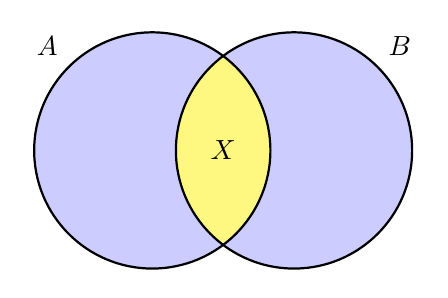
\begin{tikzpicture}[thick, set/.style = {circle, minimum size = 3cm, fill=blue!20}]

        % Set A
        \node[set,label={135:$A$}] (A) at (0,0) {};

        % Set B
        \node[set,label={45:$B$}] (B) at (1.8,0) {};

        % Intersection
        \begin{scope}
            \clip (0,0) circle(1.5cm);
            \clip (1.8,0) circle(1.5cm);
            \fill[yellow!50](0,0) circle(1.5cm);
        \end{scope}

        % Circles outline
        \draw (0,0) circle(1.5cm);
        \draw (1.8,0) circle(1.5cm);

        % Set intersection label
        \node at (0.9,0) {$X$};
    \end{tikzpicture} 
\end{center}

为了\emph{证明}这个命题,我们将引入任意固定的元素 $x \in X$。我们对它了解多少呢?我们假设 $X \subseteq A$。``$\subseteq$'' 的定义意味着 $X$ 的所有元素也是 $A$ 的元素。现在我们知道 $x$ 是 $X$ 的元素;这意味着它也是 $A$ 的一个元素。多么方便啊!我们可以对 $x$ 和 $X$ 和 $B$ 做出一些类似的陈述,这将告诉我们 $x \in B$。综上,这意味着什么?我们发现可以用 ``$\cap$'' 的定义,这告诉我们 $x \in A \cap B$。太棒了!现在,我们把它写下来。

\begin{proof}
    设 $x \in X$ 为任意固定元素。

    假设 $X \subseteq A$,根据 $\subseteq$ 的定义,可得 $x \in A$。

    同理,假设 $X \subseteq B$,可得 $x \in B$。

    因为 $x \in A$ 且 $x \in B$,根据 $\cap$ 的定义,这意味着 $x \in A \cap B$。

    综上,我们证明了当 $x \in X$ 时,$x \in A \cap B$ 也成立。由于 $x \in X$ 是任意的,因此我们得出 $X \subseteq A \cap B$ 的结论。
\end{proof}

怎么样,还不错吧?让我们看一个稍微复杂一点的例子。

\begin{proposition}
    设 $A$ 和 $B$ 为任意集合。则 $\mathcal{P}(A) \cap \mathcal{P}(B) \subseteq \mathcal{P}(A \cap B)$。
\end{proposition}

哇,这是真的吗? 回顾 \ref{sec:section3.5} 节中的问题 \ref{exc:exercises3.5.6},你会看到一个具体例子。这表明,\emph{一般而言},这一说法是正确的,而不仅仅是针对该示例。让我们找出为什么这是正确的,并证明它。

\emph{直觉}:这里有几个层次的定义共同发挥作用。特别是,幂集运算可能会让你感到困惑。关键是记住这个定义:$\mathcal{P}(A)$ 是 $A$ 的所有子集的集合。现在,这里的主要主张是一个子集关系:无论集合 $\mathcal{P}(A) \cap \mathcal{P}(B)$ 是什么(我们稍后会对其进行分析,但眼下重要的是你要立即意识到到它是什么类型的对象:集合),它应该是集合 $\mathcal{P}(A \cap B)$ 的子集。值得注意的是,这确实激发了即将到来的证明的总体形式。

甚至无需考虑 $\mathcal{P}(A) \cap \mathcal{P}(B)$ 的含义,我们就可以确定我们的证明将从``令 $X \in \mathcal{P}(A) \cap \mathcal{P}(B)$ 为任意固定集合''开始。这是因为我们需要通过获取左侧集合中的任意元素并推断它也是右侧集合中的元素来满足``$\subseteq$''的定义。这就是我们所说的证明的\textbf{结构}。

元素 $X \in \mathcal{P}(A) \cap \mathcal{P}(B)$ ``看起来像什么''?它是一个集合,并且是 $P(A)$ 和 $P(B)$ 的元素。这意味着……好吧,实际上我们现在要直接跳到正式证明,因为无论如何我们都会发现自己在下面重复相同的单词。但在继续阅读我们的证明之前,我们认为你应该尝试编写自己的证明。做完之后,你可以对比一下,看看你的做法是否正确,是不是和我们的步骤一样,写的是否清楚等等。看看你能做到什么程度!

\begin{proof}
    设 $X \in \mathcal{P}(A) \cap \mathcal{P}(B)$ 为任意固定集合。

    根据 $\cap$ 的定义,这意味着 $X \in \mathcal{P}(A)$ 且 $X \in \mathcal{P}(B)$。

    因为 $X \in \mathcal{P}(A)$,根据幂集的定义,我们知道 $X \subseteq A$。

    同理,因为 $X \in \mathcal{P}(B)$,我们知道 $X \subseteq B$。

    因为 $X \subseteq A$ 且 $X \subseteq B$,根据我们刚刚证明的引理 \ref{lemma3.9.1},可得 $X \subseteq A \cap B$。

    因为 $X \subseteq A \cap B$,根据幂集的定义,我们知道 $X \in \mathcal{P}(A \cap B)$。

    因为 $X$ 是任意固定集合,因此我们得出结论 $\mathcal{P}(A) \cap \mathcal{P}(B) \subseteq \mathcal{P}(A \cap B)$。
\end{proof}

你的证法跟上面的一样吗?你也引用了前面的引理吗?你是否在没有意识到的情况下再次证明了这个结果?把它当作一个教训!证明结果的主要好处之一是我们可以在以后的证明中使用它们!在一个证明过程中再次证明之前的结果在技术上并没有什么问题;但不重复证明会节省一点时间。如果你发现自己正在解决一个问题并发觉:“嘿,这感觉很熟悉……”,回去寻找相关的定理或引理或例子。也许你可以利用一些已经获得的知识来发挥自己的优势。

\subsection{证明 ``$=$''}

\subsubsection*{双重包含证明}

我们需要再一次回顾 ``$=$'' (在集合上下文中)的定义,因为我们将在这里频繁地使用它。

\begin{definition}
    我们说两个集合 $A$ 和 $B$ 相等,并写为 $A = B$,当且仅当 $A \subseteq B$ 且 $B \subseteq A$。
\end{definition}

就是这样!它完全是根据之前的定义 ``$\subseteq$'' 构建的(因为 ``$\supseteq$'' 的定义是完全等价的)。因此,这本身并不是一项新技术,因为它实际上是先前技术的重复应用。也就是说,要证明 $A = B$,我们只需使用上一小节中使用的技术,证明 $A \subseteq B$,然后证明 $B \subseteq A$。

事实上,这项技术非常常见,以至于被赋予了一个名字:\textbf{双重包含}。当我们以两种方式证明两个集合是彼此的子集并得出它们相等的结论时,我们将其称为\textbf{双重包含证明}。

\subsubsection*{示例}

让我们看一下双重包含技术的实际应用案例。

\begin{lemma}
    设 $A$ 和 $B$ 为任意集合。则 $A - (A \cap B) = A - B$。
\end{lemma}

\emph{直觉}:像往常一样,我们可以画一个维恩图来说服自己相信这一事实,但这并不能证明任何事情。相反,我们将采用双重包含证明。如果我们取一个元素 $x \in A - (A \cap B)$,我们可以先应用 ``$-$'' 的定义,然后应用 ``$\cap$'' 的定义,来推导出有关 $x$ 的信息。希望能够得到 $x \in A - B$。然后,如果我们取一个元素 $y \in A - B$,希望我们可以应用一些定义来推断出 $y \in A - (A \cap B)$。 也许我们还不确定具体如何做到这一点,但通过查看维恩图并使用定义,我们肯定可以弄清楚。你为什么不先尝试一下,然后再阅读我们的证明!

\begin{proof}
    我们将采用双重包含证明来证明 $A - (A \cap B) = A - B$。

    (``$\subseteq$'')首先,设 $x \in A - (A \cap B)$ 为任意固定元素。根据 ``$-$'' 的定义,我们知道 $x \in A$ 但 $x \notin A \cap B$。这意味着 $x$ 既是 $A$ 的元素又是 $B$ 的元素\emph{不}可能成立。我们已知 $x \in A$, 那么可以推导出 $x \notin B$。因此,$x \in A$ 且 $x \notin B$。根据 ``$-$'' 的定义,可以推导出 $x \in A-B$。这就证明了 $A - (A \cap B) \subseteq A - B$。


    (``$\supseteq$'')接着,设 $y \in A - B$ 为任意固定元素。根据 ``$-$'' 的定义,这意味着 $y \in A$ 且 $y \notin B$。因为 $y$ 不是 $B$ 的元素,这意味着 $y$ 当然不可能同时是 $A$ 和 $B$ 的元素。根据 ``$\cap$'' 的定义,即 $y \notin A \cap B$。因为我们知道 $y \in A$ 且 $y \notin A \cap B$,我们可以推导出 $y \in A - (A \cap B)$。这就证明了 $A - B \subseteq A - (A \cap B)$。

    综上,利用双重包含证明,我们证明出 $A - (A \cap B) = A - B$。
\end{proof}

纵观上面证明的整体结构。我们看到它分为两部分,因为它是一个双重包含证明,我们\emph{很友善地提前}向勇敢的读者指出了这一点,并将这两个部分适当地分开。从技术上讲,忽略这一点并直接深入证明也是正确的,但这可能会让读者感到困惑。证明的全部意义在于\emph{让别人信服}你已经弄清楚的事实,所以最好让他们尽可能容易地理解你正在做的事情。

让我们再看另一个证明两个集合相等的例子。这个例子会有点不同,因为双重包含的一部分将利用补集操作。作为预览,现在花一点时间思考为什么陈述 $A \subseteq B$ 和 $\overline{B} \subseteq \overline{A}$ 是\emph{等价的}(假设存在某个全集 $U$,满足 $A, B \subseteq U$)。画出维恩图并尝试举一些例子。甚至尝试证明这一点!

\begin{proposition}
    \[\Big\{x \in \mathbb{N} \mid x + \frac{8}{x} \le 6\Big\} = \{2, 3, 4\}\]
\end{proposition}

\begin{proof}
    设 $A = \Big\{x \in \mathbb{N} \mid x + \frac{8}{x} \le 6\Big\}, B = \{2, 3, 4\}$,要证明 $A = B$,我们需要证明 $A \subseteq B$ 且 $B \subseteq A$。

    首先证明 $B \subseteq A$。我们可以分别考虑这三个元素,并验证它们是否满足 A 的定义不等式:
    \begin{align*}
        2 + \frac{8}{2} &= 6 \le 6 \\
        3 + \frac{8}{3} &= \frac{17}{3} \le 6 \\
        4 + \frac{8}{4} &= 6 \le 6
    \end{align*}
    因为 $2,3,4 \in \mathbb{N}$,我们推导出 $2 \in A, 3 \in A, 4 \in A$,所以 $B \subseteq A$。

    接着证明 $A \subset B$。我们将证明 $\overline{B} \subseteq \overline{A}$,其中补集是在 $\mathbb{N}$ 作为全集的情况中获取的。也就是说,我们将证明所有自然数 $1,5,6,7,\dots$ \emph{不是} $A$ 的元素。

    为了证明这一点,我们将验证这些元素中的任何一个都\emph{不}满足 $A$ 的不等式定义。

    前两个情况很容易验证:$1 + \frac{8}{1} = 9 \nleq 6$ 且 $5 + \frac{8}{5} = \frac{33}{5} \nleq 6$。

    对于其他情况,我们可以取任意固定元素 $x \in \mathbb{N}$ 且 $x \ge 6$,此时不等式可以写为 $x + \frac{8}{x} \ge 6 + \frac{8}{x}$,因为 $\frac{8}{x} > 0$,所以 $x + \frac{8}{x} \ge 6 + \frac{8}{x} > 6$。

    这表明只有 $2,3,4$ 满足 $A$ 的不等式定义。

    综上,利用双重包含证明,我们证明出 $A = B$。
\end{proof}

仔细思考一下为什么证明后半部分采用的方法是有效的。(这实际上是条件陈述的\textbf{逆否}形式的一个实例,但我们还没有定义这些术语;我们将在下一章讨论逻辑时详细讲述。)

让我们看另一个证明集合相等的例子。这个略有不同,因为我们要证明某个集合实际上是空集,为此,我们将证明它没有元素。

\begin{proposition}
    对于每个 $n \in \mathbb{N}$,定义 $S_n = \mathbb{N}-[n]$。那么
    \[\bigcap_{n \in \mathbb{N}}S_n = \varnothing\]
\end{proposition}

如果你不理解上面式子的含义,建议你尝试几个例子。比如,看一下集合 $S_1, S_1 \cap S_2, S_1 \cap S_2 \cap S_3$ 的元素,依此类推。先尝试找出左侧大交集的候选元素,然后找出为什么它实际上不是该集合的元素。之后,尝试找出一种正式的证明并写出来; 看看下面我们是怎么做的吧!

\begin{proof}
    设 $T = \bigcap_{n \in \mathbb{N}}S_n$,便于我们后面引用它。

    要证明 $T = \varnothing$,我们需要证明 $T$ 中没有任何元素。请注意,$T$ 由许多自然数集合的交集形成,因此很明显,$T$ 中元素只可能是自然数。

    考虑任意固定元素 $x \in \mathbb{N}$,我们需要证明 $x \notin T$。

    我们知道 $x \in [x] = \{1,2,\dots, X\}$,因此根据 ``$-$'' 的定义,$x \notin \mathbb{N}-[x]$。

    根据定义,$T$ 包含属于 $\mathbb{N} - [n]$ 形式的所有集合的元素。我们已经(至少)确定了交集中的一个集合 $\mathbb{N} - [x]$,使得 $x$ 不属于该集合。因此,$x$ 不可能是 $T$ 的元素,因为它不属于所有此类集合,所以 $x \notin T$。

    因为 $x \in \mathbb{N}$ 是任意的,我们证明了 $T$ 的元素中不包含自然数,因此它根本没有元素。
\end{proof}

\emph{总结}:让我们再说明一下这项技术为何有效。我们证明 $T$ 中没有元素,即 $T \subseteq \varnothing$。这就完成了整个过程,因为 $\varnothing \subseteq T$ 无需证明,它对于任何集合都成立。因此,双重包含论证的一部分已经实现,我们可以得出 $T = \varnothing$ 的结论。

让我们再举一个例子。我们希望引入这个例子,是因为它为我们提供了使用索引集操作的进一步练习。在本节的练习中你会发现许多类似的问题。我们鼓励你尽可能多地参与其中!

\begin{proposition}
    对于每个 $n \in \mathbb{N}$,定义 $A_n = \{x \in \mathbb{R} \mid 0 \le x < \frac{1}{n}\}$。那么
    \[\bigcap_{n \in \mathbb{N}}A_n = \{0\}\]
\end{proposition}

想想这上面命题意味着什么。在数轴上画出 $A_n$ 集合的图。``$\cap$'' 有什么作用?为什么会得出 $0$ 是该交集的元素?为什么它是\emph{唯一的}元素?

``$\cap$'' 的定义在这个证明中至关重要,所以让我们回顾一下这里的定义。这里的关键词是\emph{对于每个}:

\begin{definition}
    由集合 $I$ 索引的一系列集合 $A_i$ 的交集为
    \[\bigcap_{i \in I} A_i = \{x \in U \mid x \in A_i \;\text{对于每个}\; i \in I\}\]
    其中我们假设存在集合 $U$ 满足对于每个 $i \in I, A_i \subseteq U$。
\end{definition}

也就是说,请记住,多个集合的索引交集将属于所有组成集合的元素聚合在一起。因此,在下面的证明中,你将看到我们需要证明
\begin{enumerate}[label=(\arabic*)]
    \item $0$ 确实是所有 $A_n$ 集合的元素。
    \item 没有其他数字是所有集合的元素,即对于每个非零实数,我们可以找到至少一个 $A_n$ 集合,使得该数字不是该集合的元素。
\end{enumerate} 

\begin{proof}
    首先,我们来证明
    \[\{0\} \subseteq \bigcap_{n \in \mathbb{N}}A_n\]
    这需要我们证明对于每个 $n \in \mathbb{N}, 0 \in A_n$。

    设 $n \in \mathbb{N}$ 为任意固定元素。注意,不等式 $0 \le 0 \le \frac{1}{n}$ 必然成立。

    (注:你可能会担心,因为``在极限内'' $0$ 不会``同时''小于每个分数 $\frac{1}{n}$,但这不是重点!正确的思路是:$0 \in A_1$ 吗?是的,因为 $0 \le 0 < 1$。$0 \in A_2$ 吗?是的,因为 $0 \le 0 < \frac{1}{2}$。$0 \in A_3$ 吗?是的,因为 $0 \le 0 < \frac{1}{3}$。依此类推。该不等式对于每个 $n \in N$ 分别成立,所以 $0$ 是每个此类集合的元素。如果你不担心这一点,没关系!继续前进!)

    因此,对于每个 $n \in \mathbb{N}, 0 \in A_n$,所以根据 ``$\cap$'' 的定义 $\displaystyle{0 \in \bigcap_{n \in \mathbb{N}} A_n}$。这就证明了 $\displaystyle{\{0\} \subseteq \bigcap_{n \in \mathbb{N}} A_n}$。

    接着,我们来证明
    \[\bigcap_{n \in \mathbb{N}}A_n \subseteq \{0\}\]
    我们将通过设 $\mathbb{R}$ 为全集的情况下考虑这些集合的\emph{补集}来做到这一点。具体来说,我们将证明
    \[\overline{\{0\}} \subseteq \overline{\bigcap_{n \in \mathbb{N}}A_n}\]
    这意味着我们要证明每个非零实数\emph{不是每个} $A_n$ 的元素。

    设 $x \in \mathbb{R}$ 为任意固定元素,且 $x \ne 0$。也就是说,要么 $x > 0$ 要么 $x < 0$。我们加下来将分这两种情况讨论。

    \emph{情况 1}:假设 $x > 0$。考虑实数 $\frac{1}{x} \in \mathbb{R}$。由于 $\mathbb{R}$ 中的自然数是无限且无界的,因此我们可以选择一个\emph{大于}该实数的自然数 $M$。也就是说,我们可以选择 $M \in \mathbb{N}$ 使得 $M > \frac{1}{x}$。

    (注意:想想为什么会这样。我们还没有\emph{证明} $\mathbb{N}$ 是无限的,或者数字沿着 $\mathbb{R}$ 的数轴``永远延续下去'',但我们希望这些想法对你来说直观且合理。)

    取 $M \in \mathbb{N}$ 且 $M > \frac{1}{x}$。由于 $x > 0$,我们可以将不等式两边同时乘以 $x$;由于 $M > 0$(因此 $\frac{1}{M} > 0$),我们可以再次乘以 $\frac{1}{M}$。由此得到 $x > \frac{1}{M}$。相应地,$x \ne A_M$,因为 $-\frac{1}{M} < x < \frac{1}{M}$ 为假。

    由于 $x \notin A_M$,所以 $x$ 肯定不是所有此类集合的元素。因此 $\displaystyle{x \notin \bigcap_{n \in \mathbb{N}} A_n}$

    \emph{情况 2}:假设 $x < 0$。我们采用跟前面类似的论证;这次,我们只考虑 $-x$,因为 $-x > 0$。使用与上面相同的逻辑,我们肯定可以找到满足 $M > \frac{1}{-x} = -\frac{1}{x}$ 的自然数 $M \in \mathbb{N}$。整理不等式可得 $x < -\frac{1}{M}$。因此 $x \notin A_M$,所以 $\displaystyle{x \notin \bigcap_{n \in \mathbb{N}} A_n}$。

    综上,我们已经证明,任意 $x \in \mathbb{R}$ 且 $x \ne 0$ 都不是至少一个 $A_n$ 集合的元素,因此任何这样的 $x$ 都不是它们交集的元素。因此,$\displaystyle{{0} \subseteq \bigcap_{n \in \mathbb{N}} A_n}$,并且我们已经通过双重包含论证证明了该主张。
\end{proof}

这个证明比其他证明更难一些,所以请务必多阅读几次,确保你理解每个步骤的思路和内容。特别是,考虑一下我们是如何选择 $M \in \mathbb{N}$ 满足 $M > \frac{1}{x}$ 这一步的步骤。你认为我们神奇地凭直觉做出了这个选择吗?或者我们是否认识到我们希望 $x < \frac{1}{M}$ 对于某些 $M$ 成立,进一步整理不等式以找出如何实现这一点?

\subsection{证伪}

\subsubsection*{举个例子}

考虑如下命题:
\begin{center}
    对于任意集合 $F, G, H$,如果 $F \subseteq G \cup H$,则要么 $F \subseteq G$ 要么 $F \subseteq H$。
\end{center}

这种说法成立吗?如果成立,我们该如何证明呢?我们取任意固定元素 $x \in F$。由于 $F \subseteq G \cup H$,这告诉我们 $x \in G \cup H$。 相应地,$x \in G$ 或 $x \in H$。这都没错吧?我们的证明完成了吗?

我们希望你能看出来这是行不通的!特别是,我们最后还没有满足 ``$\subseteq$'' 的定义。如果我们的目标是证明 ``$F \subseteq G$ 或 $F \subseteq H$'',那么我们应该得出结论,其中一个或另一个成立:即 $F$ 的\emph{每个}元素都是 $G$ 的元素,或者 $F$ 的\emph{每个}元素都是 $H$ 的元素。

我们发现 $F$ 的每个元素本身要么是 $G$ 的元素,要么是 $H$ 的元素,但我们不能确定 $F$ 的所有元素都是 $G$ 的元素或都是 $H$ 的元素。再次通读最后两段,以确保你跟上了逻辑。可能很容易为这个命题写出一个``证据'',却没有意识到你迈出了错误的一步!

\subsubsection*{定位错误}

这种对错误的识别是我们要发展的技能之一,它将在多个方面提供帮助。你会注意到,许多练习(到目前为止有一些,但随着我们继续深入,会有更多)要求你找出某些主张``证明''中的缺陷。通过指出存在缺陷,从而帮助你获得正确的证明(或多个证明,视情况而定)。阅读在逻辑、事实和清晰度上有误的证明是一项基本技能。更重要的是,仔细阅读别人的成果必然会让你成为一个对自己的成果更加挑剔的读者,并且会帮助你发现像前面段落中那样的潜在错误。如果你没有抓住它,请不要担心;既然你已经看到了它,你将来就会留意类似的错误!正如我们所说,这项技能是不断发展起来的,到读完本书时,你将成为数学证明的出色读者和作者。

\subsubsection*{反例}

那么,现在我们该怎么办?我们刚刚意识到我们上面的``证明''不起作用。这是否意味着该说法实际上是错误的?实际上,这一切意味着(到目前为止)我们的证明尝试失败了。也许其他一些逻辑路线会神奇地把我们带到难以捉摸的结论。

或者,也许这个说法确实是错误的。我们怎样才能证明这一点?考虑一下该命题的逻辑形式:它说某些陈述对于任意集合 $F,G,H$ 都成立。它说假设 $F \subseteq G \cup H$ 总是必然意味着 $F \subseteq G$ 或 $F \subseteq H$。要证明这并不总是成立,我们只需要找到所谓的\textbf{反例}即可。

我们将在下一章形式化逻辑时再次讨论所有这些想法,但现在你需要知道的是:\textbf{反例}是一个具体的、详细的、描述性的例子,它说明了关于``每个……''或``任意……''或``皆可能……''实际上并\emph{不}适用于所有情况。反例相当于通过展示该类中\emph{不具有}该属性的一个对象来\textbf{反驳}整个类对象具有某种属性的陈述。

\subsubsection*{示例}

让我们看一下寻找和陈述反例的过程如何解决我们上面的例子。

\begin{example}
    对于任意集合 $F, G, H$,如果 $F \subseteq G \cup H$,则要么 $F \subseteq G$ 要么 $F \subseteq H$。
\end{example}

这个命题应该适用于任意集合 $F,G,H$,因此当我们描述反例时,我们最好\emph{准确地}描述这三个集合是什么。我们不能只是解释解决这个问题的方法并讨论如何可能存在具有特定属性的三个集合。我们必须通过明确定义它们来告诉读者它们到底是什么。这就是我们反驳这一主张的第一行,但我们不能直接跳到这一点,因为我们还不知道如何定义它们!

这就是工作或乐趣所在:我们需要尝试这些集合所需的属性来帮助我们想出一个例子。回想一下,我们希望这些集合满足某些属性:我们应该确保假设 $F \subseteq G \cup H$ 成立,但我们希望结论 --- $F \subseteq G$ 或 $F \subseteq H$ --- 为假。

这是意味着什么呢?好吧,我们认为你会同意,从逻辑上讲,该陈述的``相反''或``否定''是 ``$F \not\subseteq G$'' 和 ``$F \not\subseteq H$''。(\textbf{逻辑否定}的概念将在下一章中再次出现;目前,我们认为你可以通过应用指导日常生活的逻辑原则来理解它。很快,我们将正式化这一想法。)

我们现在有一个具体的目标:找到满足以下所有三个条件的三个集合 $F,G,H$:

\begin{align*}
    F &\subseteq G \cup H \\
    F &\not\subseteq G \\
    F &\not\subseteq H \\
\end{align*}

接下来需要考虑的一件事是 ``$\not\subseteq$'' 的含义。我们有 ``$\subseteq$'' 的定义,那么它的``相反''或``否定''是什么?为了使 $F \subseteq G$ 成立,我们要求 $F$ 的每个元素也是 $G$ 的元素;因此,如果不成立,那么 $F$ 中至少有一个元素不是 $G$ 的元素。同理也适用于 $F \not\subseteq H$。现在,我们可以通过应用定义以一种有用的方式重申我们的目标:

\begin{align*}
    &F \text{的每个元素都是} G \text{的元素或} H \text{的元素} \\
    &F \text{中至少有一个元素不是} G \text{的元素} \\
    &F \text{中至少有一个元素不是} H \text{的元素} \\
\end{align*}
这对于最终找到我们的反例非常有帮助!我们总结了声明的所有基本部分,并以更直观的方式重述了这些属性。剩下的工作就是在草稿纸上写写画画,看看我们能想出什么。一种方法是为 $F, G$ 和 $H$ 及其潜在的``重叠''绘制一种``空''维恩图,然后填充足够的元素以满足上述三个属性。

第一个条件要求集合 $F$ 完全``位于'' $G$ 和 $H$ 之内;但是,第二个和第三个条件要求存在 $F$ 的两个元素,其中一个不是 $G$ 的元素,另一个不是 $H$ 的元素。这就是我们要做的!你可能会说这是一个简单的例子,但我们说这是一个\emph{有效的}例子。现在让我们开始写下我们的反驳:

\begin{proof}
    下面声明为假:
    \begin{center}
        对于任意集合 $F, G, H$,如果 $F \subseteq G \cup H$,则要么 $F \subseteq G$ 要么 $F \subseteq H$。
    \end{center}
    我们将用反例来反驳该观点。

    定义 $F = \{1, 2\}, G = \{1\}, H = \{2\}$。

    请注意 $G \cup H = \{1, 2\}$。由于 $F = G \cup H$,那么当然 $F \subseteq G \cup H$。因此,该主张的假设成立。

    然而,请注意 $2 \in F$ 但 $2 \notin G$。因此,$F \not\subseteq G$。

    同样,请注意 $1 \in F$ 但 $1 \notin H$。因此,$F \not\subseteq H$。

    因此,该主张为假。
\end{proof}

该示例的一个重要教训如下:

\begin{center}
    寻找反例不一定是最有趣或最复杂的,你也不需要以某种方式描述所有可能的反例。我们只需要找到一个反例,我们需要看看它是如何运作的。
\end{center}

就是这样!这正是我们在上面的证明中所做的:我们定义了所有重要的对象(三个集合 $F,G,H$),然后指出并描述了它们具有的所有相关属性。我们并没有让读者检查反例是否有效;我们向他们展示了细节。我们并没有争论宇宙中某个地方存在这样的集合;我们只是认为宇宙中存在这样的集合。我们明确地定义了它们。

这很重要,我们希望你的反例具有与我们上面类似的证明结构。当你尝试给出反例时,大部分工作将在证明开始之前``在幕后''进行。不过,一旦你找到了反例,就像我们一样把它写出来。

\subsection{问题与练习}

口头或书面简要回答以下问题。这些题目全都基于你刚刚阅读的部分,因此如果你无法想起特定的定义、概念或示例,请返回重新阅读相应部分。确保自己在继续之前可以自信地回答这些问题,这将有助于你的理解和记忆!

\begin{enumerate}[label=(\arabic*)]
    \item $\subseteq$ 的定义是什么?我们如何用它来证明 $A \subseteq B$?
    \item 两个集合相等意味着什么?
    \item 什么是\emph{双重包含}证明?
    \item 什么是反例?
    \item 假设 $A,B,U$ 是集合,且 $A,B \subseteq U$。为什么我们可以通过证明 $\overline{B} \subseteq \overline{A}$ 来证明 $A \subseteq B$ 呢?尝试说服朋友相信这是一种有效的技术。
\end{enumerate}

\subsubsection*{试一试}

尝试回答以下简答题。这些题目要求你实际动笔写一写,或(对朋友/同学)口头描述一些东西。目的是让你练习使用新概念、定义和符号。别担心,这些题本来就很简单。确保能够解决这些问题将对你有所帮助!

\begin{enumerate}[label=(\arabic*)]
    \item 首先,\textbf{证明}如下声明:
        \begin{center}
            对于任意集合 $A,B,C$,子集关系 $A - (B - C) \subseteq (A - B) \cup C$ 成立。
        \end{center}
        接着,找到这些集合实际上总是\emph{相等}这一主张的\emph{反例}。
    \item 假设 $A,B,C$ 是集合并且 $A \subseteq B$。证明 $A \times C \subseteq B \times C$。
    \item 假设 $A \subseteq C$ 且 $B \subseteq D$。证明 $A \times C \subseteq B \times C$。
    \item 设 $A = \{x \in \mathbb{R} \mid x^2 > 2x + 8\}$ 且 $B = \{x \in \mathbb{R} \mid x > 4\}$。对于以下每个主张,要么证明它是正确的,要么提供反例来证明它是错误的。
        \begin{enumerate}[label=(\alph*)]
            \item $A \subseteq B$
            \item $B \subseteq A$
        \end{enumerate}
    \item 设 $A, B, U$ 为集合,且 $A, B \subseteq U$。通过\emph{双包含论证}证明 $A - B = A \cap \overline{B}$。
    \item 令 $S = \{x \in \mathbb{R} \mid -2 < x < 5\}$ 且 $T = \{x \in \mathbb{R} \mid -4 \le x \le 3\}$。在 $\mathbb{R}$ 作为全集的情况下,$S \cap \overline{T}$ 是什么?找到一个集合,然后使用双包含论证证明它是正确的。
    \item \textbf{证明}以下断言:如果 $A \subseteq B$,则 $\mathcal{P}(A) \subseteq \mathcal{P}(B)$。
    \item 对于每个 $n \in \mathbb{N}$ 令 $S_n = \{x \in \mathbb{R} \mid -\frac{1}{n} < x < \frac{1}{n}\}$。证明
        \[\bigcap_{n \in \mathbb{N}}S_n = \{0\}\]
    \item 设 $I = \{x \in \mathbb{R} \mid 0 < x < 1\}$。对于每个 $x \in I$,定义 $S_x = \{y \in \mathbb{R} \mid x < y < x + 1\}$。 证明
        \[\bigcup_{x \in I}S_x = \{z \in \mathbb{R} \mid 0 < z < 2\}\]
    \item 对于每个 $n \in \mathbb{N}$,定义集合 $A_n$ 和 $B_n$
        \begin{align*}
            A_n &= \Big\{x \in \mathbb{R} \mid 0 ≤ x < \frac{n - 1}{n}\Big\} \\
            B_n &= \Big\{y \in \mathbb{R} \mid -\frac{1}{n} < y < 1\Big\}
        \end{align*}
        通过双重包含论证\textbf{证明}以下集合相等:
        \[\bigcup_{n \in \mathbb{N}}A_n = \bigcap_{n \in \mathbb{N}}B_n\]
\end{enumerate}


\newpage
% !TeX root = ../../book.tex
\section{总结}

\newpage
% !TeX root = ../../book.tex
\section{本章习题}

这些问题包含了本章涵盖的所有内容,以及我们之前见过的内容,可能还有一些假设的数学知识。当然,我们并不期望你完成所有这些工作,但是你做得越多,学到就越多!请记住,不\emph{做}数学就无法真正学习数学。亲自动手解决问题。阅读一些陈述并思考它们。尝试写出证明并将其展示给朋友,看看他们是否信服。不断练习你的功力,将你的想法以清晰、精确、合乎逻辑的方式写下来。写出一个证明,然后对其进行编辑,以使其更好。最重要的是,持续不断\emph{做}数学!

标有 $\blacktriangleright$ 号的简答题仅需要解释或陈述答案,无需严格证明。

特别具有挑战性的问题带有 $\bigstar$。

\begin{exercise}
    $\blacktriangleright$ 以下关于元素和子集的陈述,请说明它们为真还是为假。准备好向持怀疑态度的朋友捍卫你的选择!
    在整个问题中,我们将使用以下定义:
    \begin{align*}
        A &= \{x \in \mathbb{Z} \mid -3 \le x \le 3\} \\
        B &= \{y \in \mathbb{Z} \mid -5 < y < 6\} \\
        C &= \{x \in \mathbb{R} \mid x^2 \ge 9\} \\
	    D &= \{x \in \mathbb{R} \mid x < -3\} \\
        E &= \{n \in \mathbb{N} \mid n \text{为偶数} \}
    \end{align*}
    \begin{enumerate}[label=(\alph*)]
        \item $A \subseteq B$
        \item $C \cap D = \varnothing$
        \item $4 \in E \cap B$
        \item $\{4\} \subseteq A \cap E$
        \item $10 \in C - D$
        \item $A \cup B \supseteq C$
        \item $3 \in A \cap C$
        \item $0 \in (A - B) \cup D$
        \item $E \cap C \subseteq \mathbb{Z}$
        \item $0 \notin B - C$
    \end{enumerate}
\end{exercise}

\begin{exercise}
    $\blacktriangleright$ 设 $m, n \in \mathbb{N}$。假设 $m \le n$。解释为什么 $\mathcal{P}([m]) \subseteq \mathcal{P}([n])$。
\end{exercise}

\begin{exercise}
    回顾 \ref{sec:section3.9} 节中的问题 \ref{exc:exercises3.9.7}。我们证明,每当两个集合满足 $A \subseteq B$ 时,它们也必然满足 $\mathcal{P}(A) \subseteq \mathcal{P}(B)$。仔细阅读该证明,提醒自己注意细节。

    这种说法``反过来''是否成立?也就是说,假设 $\mathcal{P}(A) \subseteq \mathcal{P}(B)$。你能证明 $A \subseteq B$ 也成立吗?或者你能找到一个反例吗?
\end{exercise}

\begin{exercise}
    使用``集合构建符''重写以下陈述来定义集合。然后,如果可能的话,使用大括号写出集合的所有元素;如果不能,请解释原因并写出该集合的三个示例元素。
    \begin{enumerate}[label=(\alph*)]
        \item 设 $A$ 为平方小于 $39$ 的所有自然数的集合。
        \item 设 $B$ 为方程 $x^2 - 3x - 10 = 0$ 所有实根的集合。
        \item 设 $C$ 为和为非负数的整数对的集合。
        \item 设 $D$ 为实数对的集合,其第一个坐标为正,第二个坐标为负,且两个坐标和为正。
    \end{enumerate}
\end{exercise}

\begin{exercise}
    定义如下集合:
    \begin{align*}
        A &= \{x \in \mathbb{R} \mid x^2 - x - 12 < 0 \} \\
        B &= \{y \in \mathbb{R} \mid -3 < y < 4\}
    \end{align*}
    证明 $A = B$。
\end{exercise}

\begin{exercise}
    设 $X$ 为你学校学生的集合。

    定义属性 $P(x)$ 使得 $A := \{x \in X \mid P(x)\}$ 是 $X$ 的真子集且 $A \ne \varnothing$。

    接着,定义属性 $Q(x)$ 使得 $B := \{x \in X \mid Q(x)\}$ 是 $A$ 的真子集(即 $B \subset A$)且 $B \ne \varnothing$。
\end{exercise}

\begin{exercise}
    设 $A, B, C$ 为集合且 $A \subseteq C, B \subseteq C$。
    \begin{enumerate}[label=(\alph*)]
        \item 绘制集合 $\overline{A} \cap \overline{B}$ 和 $\overline{(A \cap B)}$ 的维恩图。
        \item 证明 $\overline{A} \cap \overline{B} \subseteq \overline{(A \cap B)}$。
        \item 定义特定集合 $A,B,C$,使其严格包含,即 $\overline{A} \cap \overline{B} \subset \overline{(A \cap B)}$
        \item 定义特定集合 $A,B,C$,使得 $\overline{A} \cap \overline{B} = \overline{(A \cap B)}$。
    \end{enumerate}
\end{exercise}

\begin{exercise}
    令 $S = \{(m, n) \in \mathbb{Z} \times \mathbb{Z} \mid m = n^2\}$。$S$ 与集合 $T = \{(m, n) \in \mathbb{Z} \times \mathbb{Z} \mid n = m^2\}$ 的关系如何?如果一个是另一个的子集,请证明它。如果不是,请提供示例来证明这一点。
\end{exercise}

\begin{exercise}
    令 $(a,b)$ 为笛卡尔平面上的一点,即 $(a,b) \in \mathbb{R} \times \mathbb{R}$。设 $\varepsilon$(希腊字母 \emph{epsilon})为非负实数,即 $\varepsilon \in \mathbb{R}$ 且 $\varepsilon \ge 0$。

    设 $C_{(a,b),\varepsilon}$ 为``接近'' $(a, b)$ 的实数集合,定义如下:
    \[C_{(a,b),\varepsilon} = \Big\{(x, y) \in \mathbb{R} \times \mathbb{R} \mid \sqrt{(x - a)^2 + (y - b)^2} < \varepsilon\Big\}\]
    \begin{enumerate}
        \item 给出集合 $C_{(a,b),\varepsilon}$ 的几何描述。\\
        当我们改变 $a$ 和 $b$ 时,集合会发生什么?\\
        当我们改变 $\varepsilon$ 时会发生什么?
        \item $C_{(0,0),1} \cap C_{(0,0),2}$ 是什么?
        \item $C_{(0,0),1} \cup C_{(0,0),2}$ 是什么?
        \item $C_{(0,0),1} \cap C_{(2,2),1}$ 是什么?
    \end{enumerate}
\end{exercise}

\begin{exercise}
    考虑如下(错误)声明:
    \[\bigcup_{n \in \mathbb{N}}\mathcal{P}([n]) = \mathcal{P}(\mathbb{N})\]
    \begin{enumerate}[label=(\alph*)]
        \item 下面``证明''有什么问题?指出错误并解释为什么它/它们破坏了``证明''。
            \begin{spoof}
                首先证明 $\displaystyle{\bigcup_{n \in \mathbb{N}}\mathcal{P}([n]) \subseteq \mathcal{P}(\mathbb{N})}$

                考虑左侧并集的任意元素 $X$。

                根据索引并集的定义,我们知道存在 $k \in \mathbb{N}$ 使得 $X \subseteq [k]$。

                由于 $[k] \subseteq \mathbb{N}$,并且 $X \subseteq [k]$,我们推断出 $X \subseteq \mathbb{N}$。

                因此 $X \in \mathcal{P}(\mathbb{N})$。

                接着我们证明 ``$\subseteq$'' 关系在另一个方向上也成立。

                考虑任意元素 $Y \subseteq \mathbb{N}$。

                根据子集的定义,以及 $Y$ 是自然数的集合,我们知道存在 $\mathscr{l} \in \mathbb{N}$ 使得 $Y \subseteq [\mathscr{l}]$。

                根据索引并集的定义,我们知道 $\displaystyle{Y \in \bigcup_{n \in \mathbb{N}}\mathcal{P}([n])}$。

                由于我们已经证明了 $\subseteq$ 和 $\supseteq$,所以我们知道这两个集合是相等的。
            \end{spoof}
            $\quad$
        \item 通过定义集合 $S$ 的\textbf{明确}示例来反驳该主张,使得
            \[S \in \mathcal{P}(\mathbb{N}) \qquad \text{且} \qquad S \notin \bigcup_{n \in \mathbb{N}}\mathcal{P}([n])\]
    \end{enumerate}
\end{exercise}

\begin{exercise}
    设 $A = [3] \times [4]$。(记住 $[n] = \{1, 2, 3, \dots , n\}$。)
    设 $B = \{(x, y) \in \mathbb{Z} \times \mathbb{Z} \mid 0 \le 3x - y + 1 \le 9\}$。
    \begin{enumerate}[label=(\alph*)]
        \item \textbf{证明} $A \subseteq B$。
        \item $A = B$ 吗?为什么相等或者为什么不等?请\textbf{证明}你的主张。
    \end{enumerate}
\end{exercise}

\clearpage

\begin{exercise}
    令 $n \in \mathbb{N}$ 为固定自然数。设 $S = [n] \times [n]$。 设 $T$ 为集合
    \[T =\Big\{(x, y) \in \mathbb{Z} \times \mathbb{Z} \mid 0 \le nx + y - (n + 1) \le n^2 - 1\Big\}\]
    证明 $S \subseteq T$ 但 $S \ne T$。
\end{exercise}

\begin{exercise}
    假设 $A$ 和 $B$ 为集合。
    \begin{enumerate}[label=(\alph*)]
        \item \textbf{证明} 
        \[\mathcal{P}(A) \cup \mathcal{P}(B) \subseteq \mathcal{P}(A \cup B)\]
        \item 给出 $A$ 和 $B$ 的\textbf{明确}示例,其中 (a) 中的包含是\textbf{严格包含}。
    \end{enumerate}
\end{exercise}

\begin{exercise}
    设 $S$ 和 $T$ 为集合,其元素本身也是集合。假设 $S \subseteq T$,\textbf{证明} 
    \[\bigcup_{X \in S} X \subseteq \bigcup_{Y \in T} Y\]
\end{exercise}

\begin{exercise}
    设 $A, B, C, D$ 为集合。
    \begin{enumerate}[label=(\alph*)]
        \item \textbf{证明} 
        \[(A \times B) \cup (C \times D) \subseteq (A \cup C) \times (B \cup D)\]
        \item 给出 $A,B,C,D$ 的\textbf{明确}示例,其中 (a) 中的包含是\textbf{严格包含}。
    \end{enumerate}
\end{exercise}

\begin{exercise}
    设 $A, B, C$ 为集合。证明
        \[A \times (B \cap C) = (A \times B) \cap (A \times C)\]
    和
        \[A \times (B - C) = (A \times B) - (A \times C)\]
\end{exercise}

\begin{exercise}
    设 $X,Y,Z$ 为集合。证明 $(X \cup Y ) - Z \subseteq X \cup (Y - Z)$ 但\emph{不一定}相等。
\end{exercise}

\begin{exercise}
    找出集合 $S$ 的示例,使得 $S \in \mathcal{P}(\mathbb{N})$ 且 $S$ 恰好拥有 $4$ 个元素。
    接着找出集合 $T$ 的示例,使得 $T \subseteq \mathcal{P}(\mathbb{N})$ 且 $T$ 恰好拥有 $4$ 个元素。
\end{exercise}

\begin{exercise}
    找出集合 $R,S,T$ 的示例,使得 $R \in S$ 且 $S \in T$ 且 $R \subseteq T$ 但 $R \notin T$。
\end{exercise}

\begin{exercise}
    确定以下每集合是什么,并证明你的主张。
    \[\bigcap_{n \in \mathbb{N}}[n] \qquad \text{和} \qquad \bigcup_{n \in \mathbb{N}}[n]\]
\end{exercise}

\begin{exercise}
    设 $I = \{-1, 0, 1\}$。对于每个 $i \in I$,定义 $A_i = \{i - 2, i - 1, i, i + 1, i + 2\}$ 和 $B_i = \{-2i, -i, i, 2i\}$。
    \begin{enumerate}[label=(\alph*)]
        \item 写出 $\displaystyle{\bigcup_{i \in I}A_i}$ 的元素。
        \item 写出 $\displaystyle{\bigcap_{i \in I}A_i}$ 的元素。
        \item 写出 $\displaystyle{\bigcup_{i \in I}B_i}$ 的元素。
        \item 写出 $\displaystyle{\bigcap_{i \in I}B_i}$ 的元素。
        \item 利用上面的答案,写出 $\displaystyle{\Big(\bigcup_{i \in I}A_i\Big) - \Big(\bigcup_{i \in I}B_i\Big)}$ 的元素。
        \item 利用上面的答案,写出 $\displaystyle{\Big(\bigcap_{i \in I}A_i\Big) - \Big(\bigcap_{i \in I}B_i\Big)}$ 的元素。
        \item 写出 $\displaystyle{\bigcup_{i \in I}(A_i - B_i)}$ 的元素。与 (e) 的答案有何区别?
        \item 写出 $\displaystyle{\bigcap_{i \in I}(A_i - B_i)}$ 的元素。与 (f) 的答案有何区别?
    \end{enumerate}
\end{exercise}

\begin{exercise}
    在这道题中,我们要``证明''负整数的存在性!我们说``证明''是因为直到后来我们才会真正理解我们所做的事情,但是,相信我们,这就是我们正在做的事情。

    由于这个目标,你不能\textbf{假设}存在任何严格小于 $0$ 的整数,因此你的代数步骤,尤其是 (d) 部分,不应涉及任何可能为负的项。

    也就是说,如果考虑这样的方程
    \[x + y = x + z\]
    我们\textbf{可以}通过两边同时减 $x$ 推导出 $y = z$,因为 $x - x = 0$。但是,如果我们考虑的是这样的方程
    \[x + y = z + w\]
    我们\textbf{不能}推导出 $x - z = w - y$。也许 $y > w$,所以 $w - y$ 在我们的上下文中不存在……

    设 $P = \mathbb{N} \times \mathbb{N}$。将集合 $R$ 定义为
    \[R = \{((a, b),(c, d)) \in P \times P \mid a + d = b + c\}\]
    \begin{enumerate}[label=(\alph*)]
        \item 找出三个不同的 $(c, d)$ 对,使得 $((1, 4),(c, d)) \in R$。
        \item 设 $(a, b) \in P$。证明 $((a, b),(a, b)) \in R$。
        \item 设 $((a, b),(c, d)) \in R$。证明 $((c, d),(a, b)) \in R$。
        \item 假设 $((a, b),(c, d)) \in R$ 且 $((c, d),(e, f)) \in R$。证明 $((a, b),(e, f)) \in R$。
    \end{enumerate}
\end{exercise}

\newpage
% !TeX root = ../../book.tex
\section{展望}